\documentclass[oneside, 12pt, openany]{book}

% Fonts
\usepackage[sfdefault]{atkinson} % For using a Atkinson Hyperlegible font
\usepackage[T1]{fontenc}

\usepackage[english]{babel} % English writing
\usepackage[utf8]{inputenc} % UTF8 encoding

\usepackage{graphicx} % Graphics and images
\graphicspath{ {img/} } % Images route
\usepackage{wrapfig} % Text and images in the same paragraph 

\usepackage[a4paper,top=30mm,left=30mm,right=25mm,bottom=35mm,headheight=55mm, footskip=20mm]{geometry} % Margin configuration

% Format packages
\usepackage{titlesec}
\usepackage{setspace}
\usepackage{ragged2e}
\usepackage{fancyhdr}
\usepackage{lastpage}
\usepackage{stackengine}
\usepackage{array}
\usepackage{url}
\usepackage{float}
\usepackage{multirow}
\usepackage{lastpage}
\usepackage{lscape}

% Links and references
\usepackage{hyperref}
\setcounter{tocdepth}{4} % Depth of the table of contents

\hypersetup
{
    bookmarksnumbered,
    breaklinks=false,
    linktocpage=false,
    colorlinks=true,
    linkcolor=black,
    citecolor=black,
    urlcolor=red,
    menucolor=black
}

% Color package
\usepackage[table,xcdraw,dvipsnames]{xcolor}

% Include pages from another PDF
\usepackage{pdfpages}

% Text generation package
\usepackage{lipsum}

% Table generator package
\usepackage{tabularx}

% List management package
\usepackage{enumitem}

% Captions package
\usepackage{caption} 
\captionsetup[table]{skip=10pt}

% Quotes packages
\usepackage{csquotes}
\usepackage{epigraph}

% Math packages
\usepackage{amsmath}

% Algorithm packages
\usepackage{algorithm}
\usepackage{algpseudocode}

% Code packages
\usepackage{listings}

% Loads the configuration tex file
\setcounter{secnumdepth}{4} % For numbering subsubsections

% Section names format
\titleformat{\chapter}[block]
{\normalfont\Huge\bfseries\singlespacing}{\thechapter}{1em}{\Huge}
\titlespacing*{\chapter}{0pt}{-62pt}{0pt}

\titleformat{\section}[block]
{\normalfont\large\bfseries}{\thesection}{4pt}{\large}
\titlespacing*{\section}{0pt}{\baselineskip}{0pt}

\titleformat{\subsection}[block]
{\normalfont\normalsize\bfseries}{\thesubsection}{4pt}{\normalsize}
\titlespacing*{\subsection}{0pt}{0pt}{0pt}

\titleformat{\subsubsection}[block]
{\normalfont\normalsize\bfseries}{\thesubsubsection}{4pt}{\normalsize}
\titlespacing*{\subsubsection}{0pt}{0pt}{0pt}


% Header and footer format
\fancyhf{} % Clear every field

\fancyhead[L]{\bfseries{\large TODO: uniovi img}}
\fancyhead[C]{\bfseries{\large \documentname}}
\fancyhead[R]{\bfseries{\large TODO: eii img}}

\fancyfoot[CE,CO,LE,LO,RE,RO]{} % Clear all footers
\fancyfoot[C]
{
    \begin{tabular}{|ll|c}
        \hline
        \multicolumn{3}{|l|}{\tfg} \\ 
        \hline
        \textbf{Author:} Hugo Fonseca Díaz & & 
        \multicolumn{1}{c|}{
            \multirow{3}{*}
            {
                Page \thepage \hspace{1pt} of {\hypersetup{linkcolor=black} \pageref*{LastPage}}
            }
        } \\ 
        \cline{1-2}
        \textbf{Supervisors:} Raúl Mencía Cascallana, Carlos Mencía Cascallana & & \multicolumn{1}{c|}{} \\
        \cline{1-2}
        \documentdate & \version & \multicolumn{1}{c|}{} \\
        \hline
    \end{tabular}
}

\renewcommand{\headrulewidth}{0.5pt}
\renewcommand{\footrulewidth}{0pt}

% Plain rewrite for having the same header and footer in all pages
\fancypagestyle{plain}
{

    % Header and footer format
    \fancyhf{} % Clear every field

    \fancyhead[L]{\bfseries{\large TODO: uniovi img}}
    \fancyhead[C]{\bfseries{\large \documentname}}
    \fancyhead[R]{\bfseries{\large TODO: eii img}}

    \fancyfoot[CE,CO,LE,LO,RE,RO]{} % Clear all footers
    \fancyfoot[C]
    {
        \begin{tabular}{|ll|c}
            \hline
            \multicolumn{3}{|l|}{\tfg} \\ 
            \hline
            \textbf{Author:} Hugo Fonseca Díaz & & 
            \multicolumn{1}{c|}{
                \multirow{3}{*}
                {
                    Page \thepage \hspace{1pt} of {\hypersetup{linkcolor=black} \pageref*{LastPage}}
                }
            } \\ 
            \cline{1-2}
            \textbf{Supervisors:} Raúl Mencía Cascallana, Carlos Mencía Cascallana & & \multicolumn{1}{c|}{} \\
            \cline{1-2}
            \documentdate & \version & \multicolumn{1}{c|}{} \\
            \hline
        \end{tabular}
    }

    \renewcommand{\headrulewidth}{0.5pt}
    \renewcommand{\footrulewidth}{0pt}

}


\pagestyle{fancy}
\restylefloat{table}

% Captions config
\floatstyle{plaintop}
\restylefloat{table}


% Variable config
\newcommand{\documentname}{Index}
\newcommand{\version}{\textbf{Version:} 1.0}
\newcommand{\documentdate}{\textbf{Date:} Appril 16\textsuperscript{th}, 2022}
\newcommand{\tfg}{TODO: TFG Full name}
\setcounter{chapter}{-1}




% Document starts
\begin{document}


% Documentation cover page

% Front cover
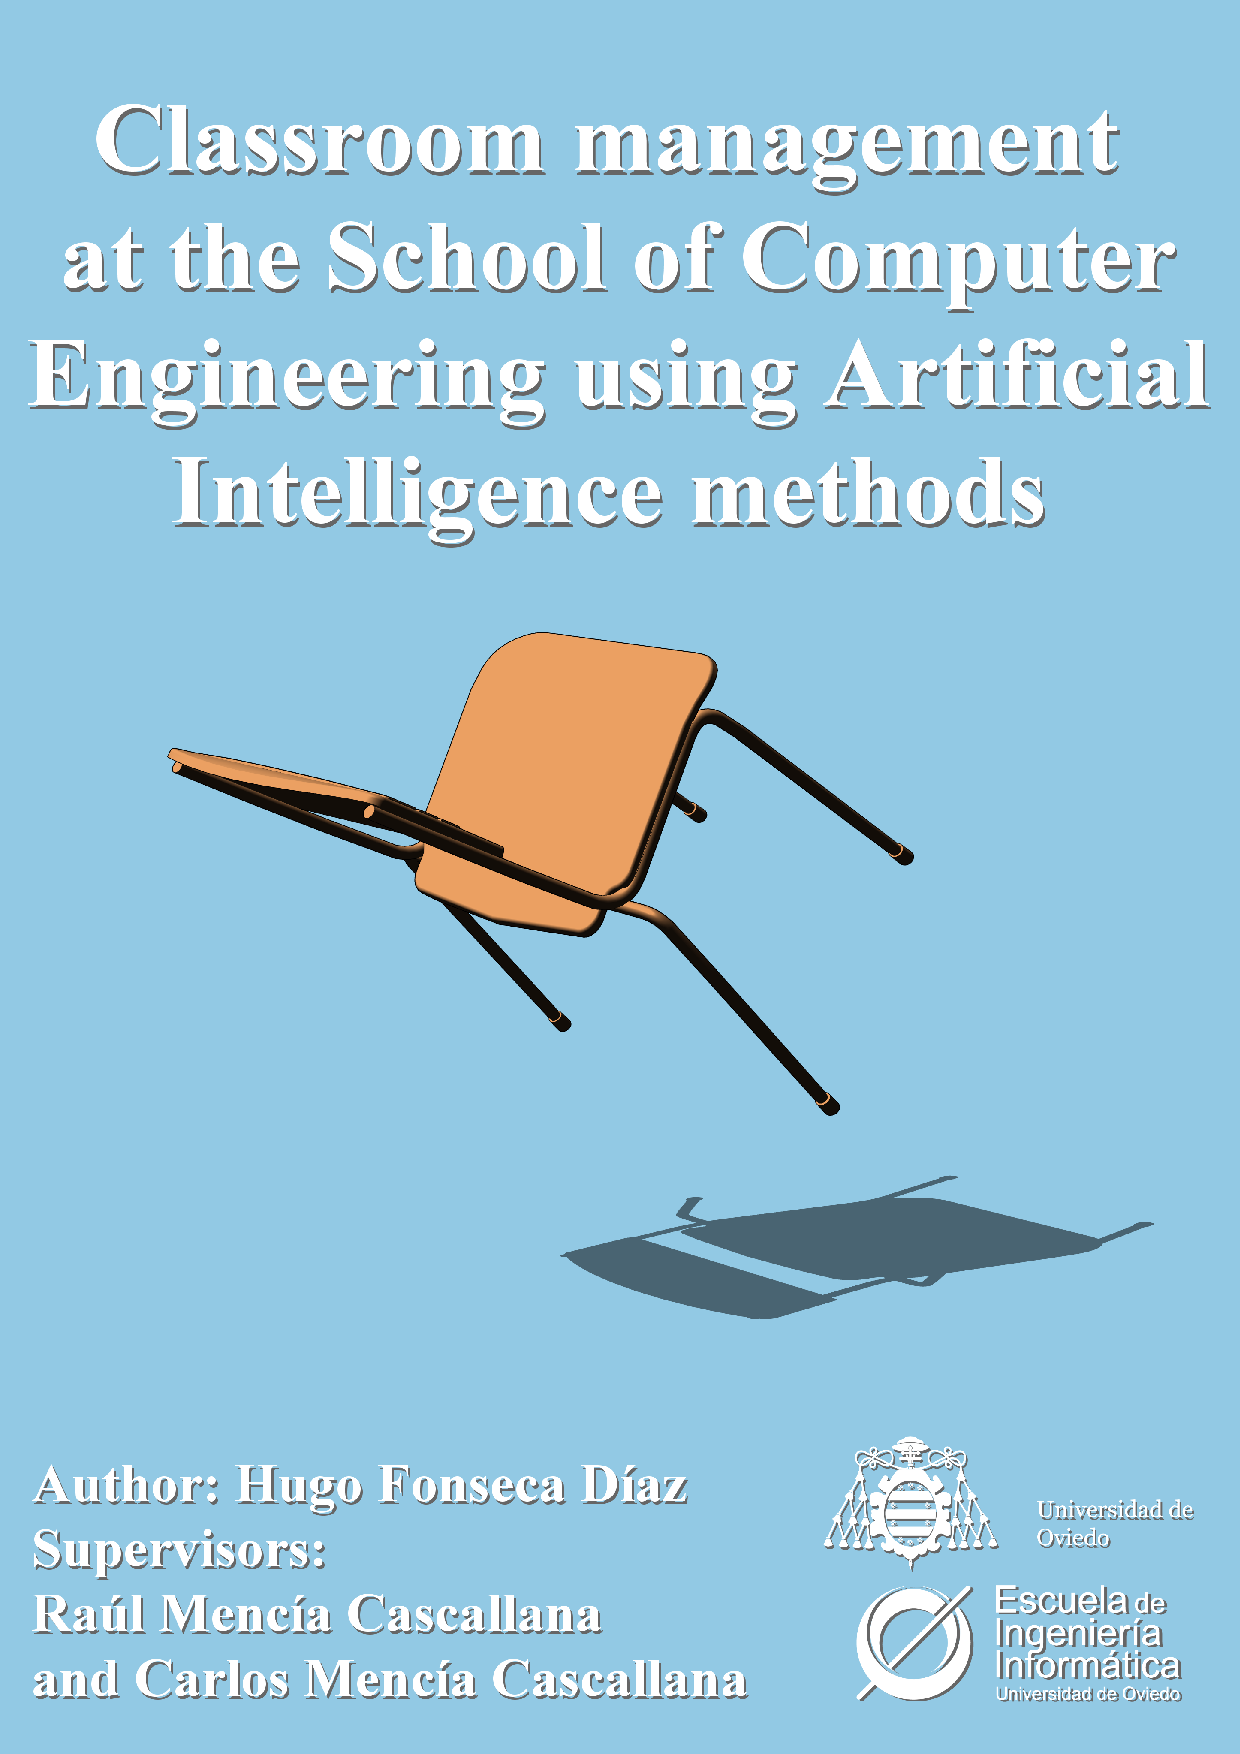
\includepdf[pages=1]{other/covers.pdf}




\renewcommand{\contentsname}{\empty}
\renewcommand{\documentname}{Index}


\chapter{Index}

\begingroup
\let\clearpage\relax

\vspace{5mm}

% Index
\tableofcontents

% List of figures
\newpage
\listoffigures

% List of tables
\newpage
\listoftables

% List of algorithms
\newpage
\listofalgorithms

\endgroup


\justify % Justify text
\setlength{\parskip}{\baselineskip} % Separate paragraphs by one line
\onehalfspacing


% Content block
{
    % Links in the content block appear in blue
    \hypersetup{linkcolor=blue}

    \newpage
    \renewcommand{\documentname}{Overview}

\chapter{Overview}

This document presents all the important information regarding the \textit{\tfg} end-of-degree thesis.

It is important to note that the structure of the contents for this document is done following the criteria and recommendations of the template document for Degree's and Master's Thesis of the School of Computing Engineering of Oviedo (version 1.4) \cite{redondotemplate} by Redondo. However, some additional chapters were introduced in order to capture the particularity of the work carried out, inspired by the research of de la Cruz \cite{delacruz18metaheuristics}.

\begin{description}

    \item \textbf{Report}. This is the chapter where I explain the personal motivation to take on this project, as well as give a brief explanation on the nature of the project and what it covers. 

    \item \textbf{Introduction}. Here we explain in a simple way the problem we want to solve, what reasons are behind the development of the project and give a description of the current situation of the School with regard to this and other similar problems.

    \item \textbf{Theoretical aspects}. The first chapter delving into the theory supporting the developed system. One example of an assignment problem is presented and solved using a greedy algorithm and a genetic algorithm, which helps to better internalize the concepts.

    \item \textbf{Problem definition}. Here the formulation of the problem as an assignment problem is elaborated. 

    \item \textbf{Proposed solution}. This chapter lays down in detail the proposed solution to the previously defined assignment problem by means of a genetic and greedy algorithms.

    \item \textbf{Project planning and budget overview}. For the planning, the Gantt chart of the project is shown, as well as the work breakdown structure. The internal and client budgets are presented, but not how they were calculated. That goes in the budget section.

    \item \textbf{Analysis}. An analysis of the system, with the system requirements, draft diagrams, use cases and the test plan specification. 

    \item \textbf{System design}. The technical details of the system analysed in the previous section. Here we include the finalised diagrams, as well as the arquitecture of the system and the in-depth test plan.

    \item \textbf{System implementation}. Details of the development of the software. The programming languages, standards and tools used to code the system, and all the relevant information gathered in the process of creating the system.

    \item \textbf{Test development}. A rundown of all the testing done for the system, with explanations for every test and the obtained results. 

    \item \textbf{Experimental results}. The conclusions reached after experimenting with different input data and the optimal configuration for the genetic algorithm's parameters. 

    \item \textbf{System manuals}. All the manuals for the system, with screenshots and guided steps meant to help the target audience for each document. 

    \item \textbf{Conclusions and future work}. The conclusions after the implementation of the project are given, as well as a list of possible improvements and new functionalities for the prototype. 

    \item \textbf{Budget}. Here we give the full details for the elaboration of the internal and client budgets, with all the intermediate steps that led us to that result. 

    \item \textbf{Annexes}. The glossary of definitions and abbreviations and a small commentary on the submitted files.

    \item \textbf{Source code}. The \textit{javadoc} of the software developed. 

\end{description}

 

    \newpage
    \renewcommand{\documentname}{Introduction}

\chapter{Introduction}


The School of Computing Engineering of the University of Oviedo has more than twenty classrooms, including theory classrooms and laboratory classrooms. Each semester there are over three hundred groups, each with their type (theory, seminar or laboratory), subject and schedule. The timetable of the groups varies on a weekly basis, this means that not all groups have to attend classes all weeks, and some of them do not even have repeating patterns.

This makes assigning classrooms to groups a complicated task, since there can be no temporal collisions. When various other constraints enter the equation, such as minimising the number of labs used by a subject or assigning classrooms to Spanish groups that are different from English groups, things become much more complex.

All this assignments are done \textit{manually} by one person. The number of enrolled students can only be \textit{guessed} when this process is done. This means that groups can be created, modified or removed once the semester has already started, so more assignments are usually made, checking once again all the restrictions. These new assignments are difficult to manage as there is not much room for flexibility to change those made before the semester. This is due to the fact that both students and teachers already use the initial assignments as a reference.

This project provides the supervisor of this process with a tool to help them calculating the assignments, reducing their workload. Not only does it generate assignments for all the groups of the semester, but can use previous assignments, total or partial, to calculate a subset of assignments (for example, the assignments for the new groups created in the middle of the semester). On top of that, the prototype developed in this thesis makes finding a set of free classrooms to hold events easy and fast, using the assignments generated previously by the system itself.


\section{Situation overview}

At the beginning of each semester, the School opens a process in which the person in charge takes the list of groups for the semester, their schedules and the list of classrooms, and performs a manual compilation of all the assignments.

There are a number of other similar procedures, like the creation of the exam timetable or the assignments of enrolled students to subject groups. However, some are not manual, but automated by a system, like the previously mentioned procedure of assigning students to groups. Seeing the potential of such tools, I was given the task of automating the assignment of classrooms to subject groups by similar means. 

The procedure of assigning the classrooms is done after configuring the student groups for the semester and knowing their schedules. Even though it is a manual process, the supervisor does not start making the assignments from scratch. First, they have the knowledge of previous years, and then they have a list of preferences or premade assignments. For example, certain laboratories can only be assigned to specific groups, like the ones from the Electronic Technology of Computers subject. The system described in this document preserves these sources of information and builds on top of them.


\section{Purpose}\label{purpose}

This project aims to help the personnel of the School manage their classrooms. It will address two main functionalities, the automation of the process of assigning classrooms to all the groups of a given semester (starting from scratch or using a previous partial or total assignment), and a tool that searches for gaps in a previous set of assignments for single or multi-day events in one or more classes.

The implementation of this system is intended to assist in the work of the supervisor for this process, and provide an efficient and flexible tool that expands the possibilities of such work. To do so, the program executes two algorithms, a genetic algorithm guided by a greedy algorithm. For a more detailed view on these algorithms the reader might refer to \ref{theory}. Once the assignments have been calculated, the system will allow the users to find classrooms to hold specific events in the middle of the semester.

Along with the system, the system manuals are submitted. These have the purpose of teaching how to install, use, maintain and extend the system. Apart from the manuals, another tool to generate the necessary files for the program is handed.


\section{Scope}

The project needs to formally define the problem of assigning classrooms of the School to all the groups of the semester, conduct a study on the problem and propose a solution. 

A development of a software prototype that solves the problem is planned, designed, implemented and tested. This prototype will solve the two main functionalities indicated in \ref{purpose} and will consist of a command line application that takes input data in plain text files and outputs the solution to plain text files. The program is configured by different configuration files depending on the functionality being executed. An experimental study on the results of the software system is carried out, finding the most fitting default values for the configuration files. The project also contains the system manuals of the application, which consist of the installation, usage, user and programmer manuals. 

Finally, an additional tool for automating the creation of the input files of the software is given. It uses a format agreed with the client and will use the same technical specifications of the main prototype, like the programming language and the development environment.


\section{Project goals}

We can identify from the scope the following objectives. They need to be met in order to close the project successfully:

\begin{enumerate}

    \item Formally define the problem of assigning classrooms to the groups of the School.

    \item Study the problem and the means to solve it.

    \item Define the proposed solution.

    \item Build a prototype that solves the problem using the algorithms described in the proposed solution.

        \begin{enumerate}

            \item It will receive plain text input files with the required data.

            \item It will output the solution to plain text files.

            \item It will be able to make the assignments starting from scratch or from a total or partial set of assignments.

            \item It will be able to search a set of free classrooms for a specific event in one or more days.

        \end{enumerate}

    \item Make a set of experiments to find the best default values for the configuration files.

    \item Write a set of manuals to cover the essentials of the system.

    \item Create another software tool that will automate the creation of the input plain text files for the main system.

    \item Validate solution with the users.

\end{enumerate}

 

    \newpage
    \renewcommand{\documentname}{Theoretical Aspects}

\chapter{Theoretical aspects}\label{theory}

A digital magazine Bootaku works with three freelancers. Dante, Virgil and Beatrice. Together they write a section about book reviews. Gathering data from previous sections, Bootaku wants to define and solve a problem of efficiently assign all reviews to the three critics so that the section gets the highest profit. For the assignments, Bootaku wants every book review to have one (and only one) associated freelancer. If a freelancer ends up with no reviews, the assignments are still valid if and only if the previous condition is met.


\section{Assignment problem}

The problem described before can be generalised with the following elements: 

\begin{description}
    \item A set of $n$ freelancers $f$
    \item A set of $m$ book reviews $r$
    \item An assignment matrix of $n \times m$ assignments $a_{fr}$ such that $a_{fr} = 0$ when freelancer $f$ is not assigned to book review $r$ and $a_{fr} = 1$ when freelancer $f$ is assigned to book review $r$.
    \item A profit matrix of $n \times m$ profits $p_{fr}$ which indicate the profit obtained when assigning freelancer $f$ to book review $r$ and that $p_{fr} \textgreater 0$.
    \item A valid solution is defined as a matrix of assignments where all the book reviews have a freelancer assigned to them and no book review has more than one associated freelancer.
\end{description}

The profit for all the assignments will then be:

\begin{equation}
    \scalebox{2}{$\sum_{f=1}^n \sum_{r=1}^m a_{fr} p_{fr}$}
\end{equation}

The optimal solution consists on having a set of assignments such that the sum of all the profits for the current assignments is maximised.

For example, imagine that for the next month's section, we have the following data. The information is represented by means of two sets: $F$ for the freelancers and $R$ for the reviews.

\begin{align}
    F &= \{ Dante, Virgil, Beatrice \} \\
    R &= \{ Divine Comedy, El Quijote \}
\end{align}

Then, our assignments and profits will be represented by the $A$ and $P$ matrices.

\begin{align}
    A &= 
    \begin{bmatrix}
        a_{11} & a_{12}\\ 
        a_{21} & a_{22}\\ 
        a_{31} & a_{32} 
    \end{bmatrix} \\
    P &= 
    \begin{bmatrix}
        p_{11} & p_{12}\\ 
        p_{21} & p_{22}\\ 
        p_{31} & p_{32} 
    \end{bmatrix}
\end{align}

Now, we are going to study valid and non-valid solutions. As we explained before, a solution is valid if every book review has a freelancer assigned to it, and no more than one.

We will analyse four sets of values for the A matrix:

\begin{align}
    A1 &= 
    \begin{bmatrix}
        0 & 1\\ 
        0 & 0\\ 
        1 & 0 
    \end{bmatrix} \\
    A2 &= 
    \begin{bmatrix}
        0 & 1\\ 
        1 & 0\\ 
        0 & 0 
    \end{bmatrix} \\
    A3 &= 
    \begin{bmatrix}
        0 & 0\\ 
        0 & 0\\ 
        1 & 0 
    \end{bmatrix} \\
    A4 &= 
    \begin{bmatrix}
        0 & 1\\ 
        0 & 0\\ 
        0 & 1 
    \end{bmatrix}
\end{align}

From these matrices, we can deduce that $A1$ and $A2$ are valid solutions, because they have one freelancer for each book review. We are not concerned with a freelancer having no book reviews assigned. However, a book review without an associated freelancer represents a non-valid solution. That is precisely the case for $A3$, the book review for \textit{El Quijote} has not an assigned freelancer. In the case of $A4$, the fact that \textit{El Quijote} has two freelancers assigned makes it a non-valid solution.

Now, we will give values to the $P$ matrix in order to discuss possible optimal solutions. We will compare them with the assignment matrices $A1$ and $A2$

\begin{align}
    P1 &= 
    \begin{bmatrix}
        4 & 12\\ 
        2 & 8\\ 
        7 & 11 
    \end{bmatrix} \\
    P2 &= 
    \begin{bmatrix}
        4 & 12\\ 
        15 & 8\\ 
        7 & 11 
    \end{bmatrix}
\end{align}

$P1$ y $A1$:

\begin{equation}
    \scalebox{1.2}{$Profit = \sum_{f=1}^n \sum_{r=1}^m a_{fr} p_{fr} = 1 \times 12 + 1 \times 7 = 19$}
\end{equation}

$P1$ y $A2$:

\begin{equation}
    \scalebox{1.2}{$Profit = \sum_{f=1}^n \sum_{r=1}^m a_{fr} p_{fr} = 1 \times 12 + 1 \times 2 = 14$}
\end{equation}

We can observe that for $P1$, the assignments defined in $A1$ are better than those in $A2$, because they result in a better profit. Another important thing about $A1$ is that it is the optimal solution to the problem, because it assigns the book reviews to the freelancers with the better profit value for their assigned books. Now $P2$ will be evaluated.

$P2$ y $A1$:

\begin{equation}
    \scalebox{1.2}{$Profit = \sum_{f=1}^n \sum_{r=1}^m a_{fr} p_{fr} = 1 \times 12 + 1 \times 7 = 19$}
\end{equation}

$P2$ y $A2$:

\begin{equation}
    \scalebox{1.2}{$Profit = \sum_{f=1}^n \sum_{r=1}^m a_{fr} p_{fr} = 1 \times 12 + 1 \times 15 = 27$}
\end{equation}

In the case of the profits values of $P2$, the situation is reversed. $A2$ is now the optimal solution and therefore better than $A1$.

The important thing to notice here is that the values for the $P$ matrix right now may appear as having no meaning whatsoever. But we need to think of $P$ as the results obtained from a profit funtion. Then, we can interpret $P1$ as values of profit in a context where Virgil has just expressed an opinion on social media related the \textit{Divine Comedy} and caused a massive controversy. We can then say that $P1$ is a function which gives more importance to public relations and so the profit $p_{12}$ is very low, whereas $P2$ gives more importance to views and so the profit $p_{12}$ is higher. Of course, in a real problem you know what the function is calculating, but this shows how we can add meaning to a set of symbols in order to understand the data more efficiently.

As you can imagine, this is an assignment problem. The actors that perform the jobs, in this case the freelancers that \textit{write} the reviews, are called the \textit{agents}. The \textit{tasks} to be performed are, in the Bootaku, problem the book reviews. Nevertheless, the agents in an assignment problem do not need to be persons (or even things that carry out actions), they can be machines, warehouses, or classrooms. The same can be said for the tasks.


\section{Heuristics and greedy algorithms}

One way of solving the Bootaku problem described earlier can be found in \textit{search algorithms}.


\section{Metaheuristics and genetic algorithms}



 

    \newpage
    \renewcommand{\documentname}{Problem definition}

\chapter{Problem definition}

The School of Computing Engineering of Oviedo must find a classroom for each group of a given semester. In most cases of this particular problem, just like in the Bootaku situation described in \ref{theory}, there are more \textit{tasks} (groups) than \textit{agents} (classrooms). And, in the same way, a valid solution implies that all groups have one (and only one) classroom assigned.

The data for the classrooms and groups can be represented by two sets $C$ and $G$. 

\begin{align}
    C &= \{ c_{1}, c_{2}, ..., c_{n} \}\\
    G &= \{ g_{1}, g_{2}, ..., g_{m} \}
\end{align}

Where $C$ is the set of $n$ elements representing all the classrooms of the School, and $G$ a set of $m$ elements representing the groups for a given semester.

A classroom can be a laboratory or a theory classroom. Groups, on the other hand, can be taught in English or Spanish, and have three types. Laboratory, theory and seminar groups. In this problem, because we are only interested in the classrooms that can be assigned to groups, we only consider two types. Laboratory and theory. That is, we consider that the types of classrooms are \textit{identical} to the types of groups.

\begin{align}
    T &= \{ t_{1}, t_{2}, ..., t_{p} \}\\
    L &= \{ l_{1}, l_{2}, ..., l_{q} \}
\end{align}

Therefore, each classroom $c$ and group $g$ have a type $t$. In the case of groups, they also are taught in language $l$.

Each group has a set of academic weeks and of group schedules. A group can attend classes weekly, every two weeks or on a non-trivial pattern, and may be taught on one or several days.

\begin{align}
    W_{i} &= \{ w_{i1}, w_{i2}, ..., w_{ir} \}\\
    H_{i} &= \{ h_{i1}, h_{i2}, ..., h_{is} \}
\end{align}

Therefore, every group $i$ has a set of weeks $W_{i}$ and a set of schedules $H_{i}$. A schedule consists of a triplet in the form $(DayOfTheWeek, start (hh:mm), finish (hh:mm)$.

Every group belongs to a subject.

\begin{align}
    S &= \{ s_{1}, s_{2}, ..., s_{t} \}
\end{align}

A subject $s$ is related to a subset of $G$ groups.

With these, we have defined all the data which we need in order to solve the problem. Now we will talk about the problem constraints that we have to fulfill.

For the constraints, we call \textit{hard constraints} those which are imperative for the solution to be valid, and \textit{soft constraints} the ones that reflect on the overall quality of the solution but are not mandatory.

Before introducing the constraints, two new concepts are presented. Restrictions and preferences.

\begin{align}
    R_{i} &= \{ r_{i1}, r_{i2}, ..., r_{iu} \}\\
    P_{i} &= \{ p_{i1}, p_{i2}, ..., p_{iv} \}
\end{align}

Restrictions and preferences can be positive or negative. A group $i$ must be assigned to a classroom in the set of its positive restrictions, and cannot be assigned to a classroom in the set of its negative restrictions. It is prefered that the group $i$ is assigned to a classroom in the set of its positive preferences, and preferably not in the set of its negative preferences. With that in mind, the constraints are listed next. 

\textbf{Hard constraints:}

\begin{description}
    \item Laboratory groups can only be assigned to laboratories.
    \item Theory and seminar groups can only be assigned to theory classrooms.
    \item A group cannot be assigned to a classroom whose capacity is less than the number of students in the group.
    \item A group with a set of positive restrictions must be assigned to one of those classrooms.
    \item A group with a set of negative restrictions cannot be assigned to one of those classrooms.
    \item A group cannot be assigned to a classroom if that classroom was already assigned to another group and both groups collide (they overlap in week and schedule).
\end{description}

\textbf{Soft constraints:}

\begin{description}
    \item Laboratory groups of the same subject must all attend the same laboratory classroom, and if not possible, at least minimise the number of laboratories assigned to them.
    \item Theory groups of the same name and course work in the same way, but being assigned to theory classrooms \footnote{All the groups in the School have the format \textit{subject.type.name}. For example the group \textit{Com.T.1} refers to \textit{theory} group \textit{1} of the \textit{Computability} subject. So all theory groups named 1 would be assigned to the same theory classroom, if possible.}.
    \item English and Spanish groups should go to different classrooms.
    \item Every hour a number of laboratories must be empty. To cover for emergencies.
    \item A group with a set of positive preferences should be assigned to one of those classrooms.
    \item A group with a set of negative preferences should not be assigned to one of those classrooms.
\end{description}

 

    \newpage
    \renewcommand{\documentname}{Proposed solution}

\chapter{Proposed solution}

We have already studied the theoretical concepts necessary to solve this type of problem, and we have formalised the problem to be solved. In this section we explain which components, techniques and algorithms we have designed and used to solve the problem of assigning classes to groups. To do so, we will define the search space, introduce the concepts of collisions and class filters, and comment on the pseudocode of the proposed algorithms.



\section{Search space}


\subsection{Assignments}

An assignment is a tuple which associates a group with a classroom.

\begin{equation}
    \scalebox{1.5}{$(G_{i}, C_{j})$}
\end{equation}

Because a group can only have \textit{one} classroom assigned, an assignment can be identified by the \textit{code} \footnote{The name convention previously mentioned: \textit{subject.type.name} (e.g. Com.T.1).} of the group. For example, the assignment for group SI.T.1 can be identified by the code SI.T.1 as well.

Assigning just \textit{one} classroom to each group means that the total number of assignments is calculated by the following expression.

\begin{equation}
    \scalebox{1.2}{$TotalNumberOfAssignments = \left|G\right|$}
\end{equation}

This implies that there are as many assignments as the number of groups for the semester.

\subsection{Solutions}

A \textit{solution} for this problem is represented by a set of all the assignments that must be performed for the semester. As presented in the previous section, the total number of assignments equals the total number of groups in that semester. So we have the next statement.

\begin{equation}
    Solution = \{ (G_{1}, C_{x}), (G_{2}, C_{y}), ..., (G_{m}, C_{z})) \}
\end{equation}

Where $m$ is the total number of groups and $x$, $y$ and $z$ are the index for the classrooms assigned to the groups. Note that the classrooms are not sequential (e.g $x$ could represent $C_{12}$ and $y$ represent $C_{3}$).

An \textit{empty solution} is represented by a set of all the assignments where each assignment is \textit{incomplete}. We mean that an assignment is incomplete when the group has no classroom assigned.

\begin{equation}
    IncompleteAssignment = (G_{i}, -)
\end{equation}

So, for the empty solution, we have a set with the following format.

\begin{equation}
    EmptySolution = \{ (G_{1}, -), (G_{2}, -), ..., (G_{m}, -)) \}
\end{equation}

Finally, a \textit{partial solution} is one in which not every assignment was performed, and a \textit{complete solution} is defined by a set in which all the assignments have been performed and each group has a classroom associated with it.

\subsection{States}

A \textit{state} represents a phase in the problem. There can be three states. The \textit{initial state}, which stands for the empty solution of non allocated assignments. The \textit{final state}, which represents a complete solution with all the assignments performed. And the \textit{intermediate states} portraying partial solutions.

A key concept to understand our design is the following. Although by default we start the execution of the algorithms with an initial state, it is also possible to start the execution with an intermediate state. This is because we can receive as input a partial or total solution of assignments and work from there. Now we will discuss how we can jump from one state to the next, which is normally called \textit{state expansion}.

To expand a state, one of the non performed assignments in the solution is executed. This means that every time a classroom is assigned to a group the state is being expanded. To perform an assignment, the number of possible candidates is the same as the number of classrooms. So we have the following.

\begin{equation}
    \scalebox{1.2}{$TotalNumberOfCandidates = \left|C\right|$}
\end{equation}

Nevertheless, as there exist constraints that indicate whether or not the solution is valid, there are filters which reduce the number of available classrooms for a group. This allows for optimized and easy to retrieve calculations in the execution of the greedy algorithm (this will be explained later in \ref{classroom-filters}). The important thing to note at this moment is that, because of these filters, not all states can be expanded.

\subsection{Instances}

The complexity of the calculations and completion time depend on many factors. Some of those factors follow. First, the number of groups for the semester, which directly translates into the number of assignments to be made. Second, the number of classrooms. If there are more classrooms, it is easier to avoid collisions. Obviously, the number of groups is much more volatile between semesters than the number of classes, which is likely to change very occasionally, if at all. Lastly, the case of starting the prototype with an intermediate state. This means that the set of assignments represents a partial solution given as input, and since the number of calculations decreases in direct proportion to the assignments already made, the completion time would be lower.

Because of the constraints of the problem, there are some groups where class allocations are more straightforward. For example, a group with only one positive restriction is either going to have that classroom assigned to it or, if it collides with other group, end up unallocated. This is why all the groups that just have one available classroom are assigned first. Also, the groups which have less students have more available classrooms than those with a large number of members.



\section{Collisions}

A collision is an overlap of the timetable of two different groups. For a collision to occur, the groups must clash at least once in the same week, day and time. Collisions are an essential part of this problem, as we cannot assign a classroom to a group if another group was previously associated with that classroom and both groups collide.

\subsection{Lazy Collision Matrix}\label{lcm}

Due to the large number of assignments that have to be made throughout the execution cycle of the genetic algorithm, the chosen data structures were properly analysed. This is where the \textit{Lazy Collision Matrix} comes in.

Imagine that we have the following group set.

\begin{equation}
    G = \{ G_{1}, G_{2}, G_{3} \}
\end{equation}

Then, our initial Lazy Collision Matrix would be represented by the expression below.

\begin{equation}
    LCM = \bordermatrix{
        & G_{1} & G_{2} & G_{3} \cr
        G_{1} &  & -1 & -1 \cr
        G_{2} & -1 &  & -1 \cr
        G_{3} & -1 & -1 & 
    } \qquad
\end{equation}

First of all, the diagonal is empty because we never compare one group against itself. Then, we can observe that the rest of values are defaulted to $-1$. Why? Because there are \textit{not yet evaluated}. That is the reason behind the name of the matrix. It is \textit{lazy} because the collisions are only calculated when needed.

Continuing with this example, imagine that we assign classroom $C_{x}$ to group $G_{1}$. Then, $G_{2}$ also tries to have $C_{x}$ assigned to it, so we check if both groups collide. We find out that they do, so we update the matrix.

\begin{equation}
    LCM = \bordermatrix{
        & G_{1} & G_{2} & G_{3} \cr
        G_{1} &  & 1 & -1 \cr
        G_{2} & 1 &  & -1 \cr
        G_{3} & -1 & -1 & 
    } \qquad
\end{equation}

Therefore, the values are updated with a $1$, which indicates that both groups \textit{collide}. This results in a different classroom $C_{y}$ being assigned to $G_{2}$. Now, $G_{3}$ has that classroom also available, so we check if it clashes with $G_{2}$. We learn that they do not collide, so we update the matrix again.

\begin{equation}
    LCM = \bordermatrix{
        & G_{1} & G_{2} & G_{3} \cr
        G_{1} &  & 1 & -1 \cr
        G_{2} & 1 &  & 0 \cr
        G_{3} & -1 & 0 & 
    } \qquad
\end{equation}

The value for non-collision is $0$, as observed. Because $G_{3}$ does not clash with $G_{2}$, they are both allocated in the same classroom.

We can now generalise the LCM as in the next expression.

\begin{equation}
    LCM = \bordermatrix{
        & G_{1} & G_{2} & G_{3} \cr
        G_{1} &  & g_{12} & g_{13} \cr
        G_{2} & g_{21} &  & g_{23} \cr
        G_{3} & g_{31} & g_{32} & 
    } \qquad
\end{equation}

Where a value $g_{ij}$ can be

\[
    \begin{cases}
        1\text{,} &\quad\text{if $G_{i}$ collides with $G_{j}$}\\
        0\text{,} &\quad\text{if $G_{i}$ does not collide with $G_{j}$}\\
        -1\text{,} &\quad\text{if the collision has not yet been evaluated}\\
        \epsilon\text{,} &\quad\text{otherwise}
    \end{cases}
\]

The main advantage of this design is that we do not have to calculate all collisions. For example, a collision between a laboratory group and a theory group would be pointless to calculate because they would never be allocated in the same classroom. Therefore we alleviate the number of calculations. 

As there is only one Lazy Collision Matrix, all calculations performed by the greedy algorithm across all populations in all generations are stored in just one place. This means that all collisions are being calculated only when necessary and only once. Think of the previous example. In a future iteration the greedy algorithm wants to check if groups $G_{1}$ and $G_{2}$ collide. It access the corresponding location in the LCM, and because it contains a $1$, the greedy concludes that they indeed collide. This is done with a $O(1)$ complexity, as the matrix is coded as a dictionary of dictionaries. If instead the greedy wanted to check if groups $G_{1}$ and $G_{3}$ collide, because the LCM has a $-1$ in that position, the greedy would have to perform the collision check and then update the matrix.



\section{Classroom filters}\label{classroom-filters}

A classroom filter is a function. It receives as input either the $C$ set or a subset $I \subset C$, and outputs a new subset $F \subset C$ with the available classrooms for a given group. It filters out the classrooms that do not comply with the hard constraints for that particular group (except collisions, which are calculated later with the LCM, refer to \ref{lcm}). All groups have the \textit{same} classroom filters.

For example, let us consider a group $G_{i}$ with type $T_{j}$ and $x$ students. A type filter for $G_{i}$ would remove from the result set all the classrooms with a type different from $T_{j}$. A capacity filter would then take the  set resulting from the previous type filter and use it as input. Then it would eliminate from the set all classrooms with a capacity lower than $x$ and return the new $F$ set.

This reduces the number of classrooms that the greedy has to evaluate and therefore decreases the complexity of the calculations. Furthermore, the filters are deterministic, that is, the execution of the filters of a group will always give the same results. This means that, if needed, the filters are only performed once per group per execution.

This may lead us to this question. \textit{If all classroom filters are executed only once per group every time you run the prototype, why bother using a lazy approach for storing them? Would it not be better to perform and store them in a dictionary at the start of the execution?} The answer is no. It is true that if we start from an empty solution the lazy approach does not present a big advantage. Nonetheless, in the case of partial solutions, it reduces the number of calculations. For example, if we want to assign a classroom to a new group created in the middle of the semester, the only thing we care about is if the group collides with any other group. The filters for the rest of the groups are, in that situation, irrelevant. This is due to the fact that they have already been allocated to their corresponding classrooms.


\subsection{Lazy Filter Dictionary}\label{lfd}

The filters work in a similar way to the Lazy Collision Matrix. Again, the election of the data structures is crucial to optimise the execution times. That is why the classroom filters are coded using a dictionary of sets. Once more, we will explain this with an example.

We have a $M$ set of $n$ classroom filters, three groups $G_{1}$, $G_{2}$ and $G_{3}$, and two classrooms $C_{1}$ and $C_{2}$.

\begin{align}
    M &= \{ M_{1}, M_{2}, ..., M_{n} \}\\
    G &= \{ G_{1}, G_{2}, G_{3} \}\\
    C &= \{ C_{1}, C_{2} \}
\end{align}

Then, we define the dictionary as a function $Dict: Keys \rightarrow Values \cup \{ \epsilon \}$, where $\epsilon$ is the $null$ character. That is, $\epsilon \notin Values$.

The keys are represented by the groups, so $Keys \equiv G$. The values depict the different sets of available classrooms for each group. Because the dictionary is as lazy as the LCM, the calculations are performed as needed, so the initial set of values are by default $\epsilon$. Then we can say that $Values = \{ \epsilon, \epsilon, \epsilon \}$.

Accordingly, we have the following cases.

\[
    Dict(x) =
    \begin{cases}
        \epsilon\text{,} &\quad\text{if} x = G_{1}\\
        \epsilon\text{,} &\quad\text{if} x = G_{2}\\
        \epsilon\text{,} &\quad\text{if} x = G_{3}\\
        \epsilon\text{,} &\quad\text{otherwise}
    \end{cases}
\]

We are now in the first execution of the greedy algorithm. Because we start from an empty state and not from an intermediate step, the greedy will try to assign a classroom for all groups. As a result of the values in the dictionary being $null$, the greedy knows that it must execute the filters, updating the dictionary. This is the LFD after the first execution for this case.

\[
    Dict(x) =
    \begin{cases}
        F_{1}\text{,} &\quad\text{if} x = G_{1}\\
        F_{2}\text{,} &\quad\text{if} x = G_{2}\\
        F_{3}\text{,} &\quad\text{if} x = G_{3}\\
        \epsilon\text{,} &\quad\text{otherwise}
    \end{cases}
\]

With each $F_{i} \subset C$ being the filtered classrooms for each group. Example of values for the $F$ sets follow.

\begin{align}
    F_{1} &= \{ C_{1} \}\\
    F_{2} &= \{ C_{1}, C_{2} \}\\
    F_{3} &= \{ \}
\end{align}

We can observe that the for $G_{1}$, classroom $C_{2}$ was filtered out. In the case of $G_{2}$, both classrooms comply with all constraints. And for $G_{3}$, there are no classes available. This is very important, because it implies that with these filters, $G_{3}$ will \textit{always} end up without a classroom. Therefore, a complete solution cannot be found for this case unless the filters are changed. Lastly, a final remark. We can say that from now on, until the prototype terminates, the greedy will not have to perform the filters for any of the groups again, as the results are already stored in the dictionary. 



\section{Greedy algorithm}

The greedy algorithm (see \ref{theory-greedy} for details) performs the assignments taking care not to infringe any hard constraint. To meet this objective, the LFD and the LCM are used. Its pseudocode is as follows.

\begin{algorithm}[H]
    \caption{ClassManager Greedy Algorithm}
    \begin{algorithmic}[1]
        \Procedure {GreedyAlgorithm}{assignments}
            \State {$solution\gets copy(assignments)$}
            \State {$repairs\gets \{\}$}
            \State {$solution\gets preprocess(solution)$}
            \For {$\ i \text{ from } 0 \text{ to } length(solution) - 1$}
                \If {$\ !isAssigned(A_{i})$}
                    \State {$c\gets bestClassroomFor(A_{i})$}
                    \If {$\ c \neq \epsilon$}
                        \State {$assignClassroomToGroup(c,\ A_{i},\ solution)$}
                        \State {$assignClassroomToSameGroups(c,\ A_{i},\ solution)$}
                    \Else
                        \State {$addToRepairs(A_{i},\ repairs)$}
                    \EndIf
                \EndIf
            \EndFor
            \State {$solution\gets repair(repairs,\ solution)$}
            \State \textbf{return} $solution$
        \EndProcedure
    \end{algorithmic}
\end{algorithm}

As can be noted, the algorithm receives a set of empty or partial assignments as an input parameter and returns another set with the assignments made. It iterates over all assignments and calculates those that are not already completed. It does this by obtaining the best class for an assignment, and if found, it assigns it not only to that group, but to all groups to which that group is related. So what does it mean if one group is related to another? It's simple, if the group is a lab group, the classroom is assigned to that group and to all lab groups belonging to its subject. If, on the other hand, the group is a theory group, the classroom found is assigned to that group and to all the theory groups in its course that share the same name.

If no class is found for a group, the group is added to the repair set. Groups belonging to that set are attempted to be fixed at the end of the procedure, before returning the set with the solution.


\subsection{Preprocessing}

The greedy algorithm preprocesses the input set with the assignments, working on those that are not yet complete. The first thing it looks at is whether the set of filtered classes for a given group contains only one element, i.e. whether only one class can be assigned to that group. If this is the case, an attempt is made to make the assignment directly, checking that there are no conflicts.

\begin{algorithm}[H]
    \caption{ClassManager Greedy Algorithm Preprocessing}
    \begin{algorithmic}[1]
        \Procedure {Preprocess}{solution}
            \For {$\ i \text{ from } 0 \text{ to } length(solution) - 1$}
                \If {$\ !isAssigned(A_{i})$}
                    \State {$filtered\gets filterClassroomsFor(group(A_{i}))$}
                    \If {$\ length(filtered) = 1$}
                        \State {$c\gets bestClassroomFor(A_{i})$}
                        \If {$\ c \neq \epsilon$}
                            \State {$assignClassroomToGroup(c,\ A_{i},\ solution)$}
                        \EndIf
                    \EndIf
                \EndIf
            \EndFor
            \State \textbf{return} $solution$
        \EndProcedure
    \end{algorithmic}
\end{algorithm}

We can observe that in this procedure the class found is not assigned to the groups related to the one we are evaluating, as it is done in the greedy algorithm itself later on. The reason for this is that additional assignments may cause another group with only one filtered class to remain unassigned, so priority is given to such groups.


\subsection{Heuristic}

The heuristic used by the greedy algorithm is very simple. Classes are filtered by type, capacity and constraints (positive and negative). Once filtered, they are iterated until one is found that does not cause a collision between the evaluated group and the rest of the groups previously assigned to that classroom.

\begin{algorithm}[H]
    \caption{ClassManager Greedy Algorithm Assignment Heuristic}
    \begin{algorithmic}[1]
        \Procedure {BestClassroomFor}{$A_{i}$}
            \State {$selected \gets \epsilon$}
            \State {$filtered \gets filterClassroomsFor(group(A_{i}))$}
            \For {$\ j \text{ from } 0 \text{ to } length(filtered) - 1$}
                \State {$selected \gets F_{j}$} \Comment{Filtered classroom $j$}
                \If {$\ !collisionExistsFor(group(A_{i}),\ selected)$}
                    \State {break out of the filtered classrooms \textit{for loop}}
                \EndIf
                \State {$selected \gets \epsilon$}
            \EndFor
            \State \textbf{return} $selected$
        \EndProcedure
    \end{algorithmic}
\end{algorithm}


\subsection{Repairs}

To conclude with the greedy algorithm components, we must talk about the assignment repair process, which is probably the most complex of all components. As previously explained, in the case of not finding an appropriate class for a group, such a group is put into the repair set. The repair process iterates each group in this set and tries to fix its assignment. For this purpose, it obtains the filtered classes of the group and, for each class, it obtains the groups that are in conflict with the evaluated group. If there is only one conflict for a class, the assignment of the conflicting group is removed and the class is assigned to the group under repair. Then, an attempt is made to obtain a new class for the conflicting group. If successful, both end up with an assigned class and the repair succeeds. If unsuccessful, the previous class is reassigned to the conflicting group and the process is repeated for each conflicting group in each class. If, after the execution of this process, the repair is unsuccessful, the group is finally unassigned.

The pseudocode for the repairing procedure follows.

\begin{algorithm}[H]
    \caption{ClassManager Greedy Algorithm Repairing Process}
    \begin{algorithmic}[1]
        \Procedure {Repair}{repairs, solution}
            \For {$\ i \text{ from } 0 \text{ to } length(repairs) - 1$}
                \State {$filtered \gets filterClassroomsFor(group(A_{i}))$}
                \For {$\ j \text{ from } 0 \text{ to } length(filtered) - 1$}
                    \State {$collisions \gets collisionsFor(group(A_{i}),\ F_{j})$}
                    \If {$\ length(collisions) > 1$}
                        \State {break out of the filtered classrooms \textit{for loop}} \Comment{Assignment could not be repaired.}
                    \EndIf
                    \State {$group \gets firstElement(collisions)$}
                    \State {$a \gets assignmentFor(group)$}
                    \State {$removeClassroomFromGroup(F_{j},\ a,\ solution)$}
                    \State {$assignClassroomToGroup(F_{j},\ A_{i},\ solution)$}
                    \State {$c \gets bestClassroomFor(a)$}
                    \If {$\ c \neq \epsilon$}
                        \State {$assignClassroomToGroup(c,\ a,\ solution)$} \Comment{Assignment repaired.}
                    \Else
                        \State {$removeClassroomFromGroup(F_{j},\ A_{i},\ solution)$} \Comment{Assignment could not be repaired.}
                        \State {$assignClassroomToGroup(F_{j},\ a,\ solution)$}
                    \EndIf
                \EndFor
            \EndFor
            \State \textbf{return} $solution$
        \EndProcedure
    \end{algorithmic}
\end{algorithm}



\section{Genetic Algorithm}

The Genetic Algorithm (GA) (see \ref{theory-GA} for details) generates sets of assignments, empty or partial, with different ordering. This sets are later piped into the greedy algorithm, which performs and returns the final assignments to the GA. The GA then evaluates the solution by calculating its fitness value. This is done until a predetermined time or number of generations is reached, returning the best order of assignments, that is, the best individual found.

\begin{algorithm}[H]
    \caption{ClassManager Genetic Algorithm (GA)}
    \begin{algorithmic}[1]
        \Procedure {GeneticAlgorithm}{popsize, numgen, maxTime, crossProb, mutProb}
            \State {$best\gets \epsilon$}
            \State {$currentTime\gets \text{get current time}$}
            \State {$gen\gets 0$}
            \State {$P \gets \{ \}$} 
            \For {$\ popsize \text{ times}$}
                \State {$P\gets P \cup \{ \text{new random individual} \}$}
            \EndFor
            \Repeat
                \State {$evaluate(P)$}\Comment{Calculate the fitness of all individuals.}
                \For {$\ \text{each individual } P_{i} \in P$}
                    \If {$\ best = \epsilon \text{ or } Fitness(P_{i}) > Fitness(best)$}
                        \State {$best\gets P_{i}$}
                    \EndIf
                \EndFor
                \State {$Q\gets nextGeneration(P,\ popsize,\ crossProb,\ mutProb)$}
                \State {$P\gets Q$}
                \State {$currentTime\gets \text{update time}$}
                \State {$gen\gets gen + 1$}
            \Until {$\ gen \geq numgen\ \text{ or } currentTime \geq maxTime$}
            \State \textbf{return} $best$
        \EndProcedure
    \end{algorithmic}
\end{algorithm}

This pseudocode is very similar to the general GA, except for two things. Here, instead of having a function that checks whether or not the individual represents a valid solution, our GA simply iterates through a number of generations, stopping when it reaches that number or when time runs out. The other thing in which they differ is that the operations carried out for creating the next generation are performed in a different procedure. This procedure selects the parents, checks whether or not the offspring should result from a crossover of its parents \footnote{This check is performed by calculating a random number that is compared with the crossover probability. If the selected number is lower or equal to the probability, the crossover is executed.} and also if the offspring is mutated \footnote{Same check as for the crossover operator but comparing the number with the mutation probability.}. A tournament is then performed between the two pairs of parents and children and the two best, in terms of fitness, are added to the next generation. The pseudocode for this procedure follows.

\begin{algorithm}[H]
    \caption{ClassManager GA Next Generation}
    \label{cm-ga-ng}
    \begin{algorithmic}[1]
        \Procedure {NextGeneration}{$P$, popsize, crossProb, mutProb}
            \State {$Q\gets \{ \}$}
            \For {$\ popsize / 2 \text{ times}$}
                \State {$\text{Parent } P_{a} \gets selectAndRemove(P)$}
                \State {$\text{Parent } P_{b} \gets selectAndRemove(P)$}
                \State {$\text{Child } C_{a} \gets copy(P_{a})$}
                \State {$\text{Child } C_{b} \gets copy(P_{b})$}
                \If {$\ crossProb \geq \text{random number from $0.0$ to $1.0$ inclusive}$}
                    \State {$C_{a} \gets crossover(copy(P_{a}),\ copy(P_{b}))$}
                    \State {$C_{b} \gets crossover(copy(P_{b}),\ copy(P_{a}))$}
                \EndIf
                \If {$\ mutProb \geq \text{random number from $0.0$ to $1.0$ inclusive}$}
                    \State {$C_{a} \gets mutation(copy(C_{a}))$}
                    \State {$C_{b} \gets mutation(copy(C_{b}))$}
                \EndIf
                \State {$\text{Winners } W_{a}, W_{b} \gets tournament(P_{a},\ P_{b},\ C_{a},\ C_{b})$}
                \State {$Q\gets Q \cup \{ W_{a}, W_{b} \}$}
            \EndFor
            \State \textbf{return} $Q$
        \EndProcedure
    \end{algorithmic}
\end{algorithm}

\subsection{Genome representation}

The individuals of the GA are represented by a vector chromosome of group codes. Each code uniquely identifies a group, therefore an assignment, and the genome tells the greedy algorithm in which order it must perform that assignment. The rationale behind this random ordering is clear if we think back on what we discussed about greedy algorithms. Their main flaw relies on not always finding the correct solution because they focus on local optimum instead of global ones. The GA helps the greedy by generating a bunch of different orderings and therefore testing which order gets closer to the optimal solution.

A vector chromosome looks like this. Let's say that $I$ represents an individual, represented by a set of group codes in a random order. Codes identify assignments, so they are indicated by $A_{i}$.

\begin{equation}
    I = \{ A_{1}, A_{2}, ..., A_{m}\}
\end{equation}

Where $m$ is the number of groups for that semester.

To convert the individual representation into an actual set of assignments in the specified order, we have designed a \textit{decoder}. The decoder has a dictionary given by the function $Dict: Keys \rightarrow Values \cup \{ \epsilon \}$. The group codes work as keys, and the assignments related to each group are the corresponding values. When an individual is decoded, the decoder simply takes each group code, obtains the value associated to them by looking in the dictionary, and then returns a set with the order given by the representation.


\subsection{Fitness function}

The fitness function of the GA has the following responsibilities. First, it passes the individual representation to the decoder in order to obtain the corresponding set of assignments. Then, the function gives the assignments to the greedy algorithm and receives the solution set. Finally, it returns the value resulting from applying its formula to the solution set. 

The formula of the fitness function is given by the sum of all fitness values multiplied by their corresponding fitness weights. Each fitness value represents a soft constraint described in the problem definition (see \ref{problem-definition}), and has a weight associated with it. 

The formula for the fitness function is therefore given by:

\begin{equation}
    formula = \sum_{i=1}^{n} V_{i} W_{i}
\end{equation}

Where $n$ is the number of fitness values defined, $V_{i}$ is fitness value $i$ and $W_{i}$ the weight associated with $V_{i}$.


\subsection{Operators}

We will briefly talk about the selected operators for the ClassManager GA (see \ref{theory-GA} for a more in-depth explanation of all the operators discussed here). The order and use of these operators can be clearly illustrated with the help of the pseudocode of procedure $NextGeneration$ (see \ref{cm-ga-ng}).


\subsubsection{Selection}

The GA uses Random Selection. This operator selects and removes a random individual from the population. Since at the end of the offspring creation cycle there is a tournament between parents and offspring, a random selection of individuals is perfectly valid in this case. The pseudocode of this operator is displayed in \ref{theory-ga-ransel}


\subsubsection{Crossover}

As we explained when we introduced this operator, the Order Crossover (OX) is the crossover operator for the ClassManager GA. As in our case it only returns one child per pair of parents, OX is called two times, with the positions of the parents inverted (check the $NextGeneration$ pseudocode to see what I mean), that is, parent $a$ acts as the first parent in the first run and as the second parent in the second run (and vice versa for parent $b$). See \ref{theory-ga-ox} for its pseudocode.

It is also important to note that the offspring are only created from a crossover if a random number between $0.0$ and $1.0$ is lower or equal to the predetermined crossover probability.


\subsubsection{Mutation}

For the mutation operator the GA uses Swap Mutation. This operator selects two group codes at random and swaps their positions. As in the crossover operator, the mutation only occurs if a randomly selected value is lower or equal to the mutation probability. The pseudocode for Swap Mutation is indicated in \ref{theory-ga-sm}.   


\subsubsection{Tournament}

Finally, we introduce the specific version of Tournament Selection implemented for the ClassManager GA. It differs from the generic Tournament Selection (see \ref{theory-ga-ts}) in that the candidates for the tournament are not a $t$ number of randomly selected individuals, but instead the two pairs of parents and children generated after executing the rest of operators. These four individuals are compared by their fitness and the best two survive, joining the new generation. Below we indicate the pseudocode for this version of Tournament Selection.

\begin{algorithm}[H]
    \caption{ClassManager GA Tournament Selection}
    \begin{algorithmic}[1]
        \Procedure {TournamentSelection}{A, B, C, D}
            \State {$I \gets \{ \}$}
            \State {$I \gets I \cup \{ A,\ B,\ C,\ D \}$}
            \State {sort $I$ by fitness, from highest to lowest}
            \State \textbf{return} $I_{1} \text{ and } I_{2}$
        \EndProcedure
    \end{algorithmic}
\end{algorithm}

\subsection{Parameters}

TODO: AFTER EXPERIMENTS

 

    \newpage
    \renewcommand{\documentname}{Project planning and budget overview}

\chapter{Project planning and budget overview}

So far we have discussed the theory that will function as a pillar of the software system to be developed. With this chapter we begin the sections focused on the software engineering used to define and build such a system. In this first chapter we present the planning and WBS of the software project, defining and explaining its phases, and finally showing an overview of the internal and customer budget.


\section{Planning}

The planning of the class management system, identified as Classmanager, has the following phases. They are shown with a Gantt diagram and with the WBS of the project. Due to the size of the Gantt chart, it is shown in its full version and split into phases. We operate with working hours of 3 hours on average every day of the week. 

The following phases were established for the planning: \textit{Project Management}, \textit{Analysis}, \textit{Design}, \textit{Development}, \textit{Documentation}, \textit{Experiments} and \textit{Closure}.


\begin{figure}[H]
    \caption{WBS}
  \centering
  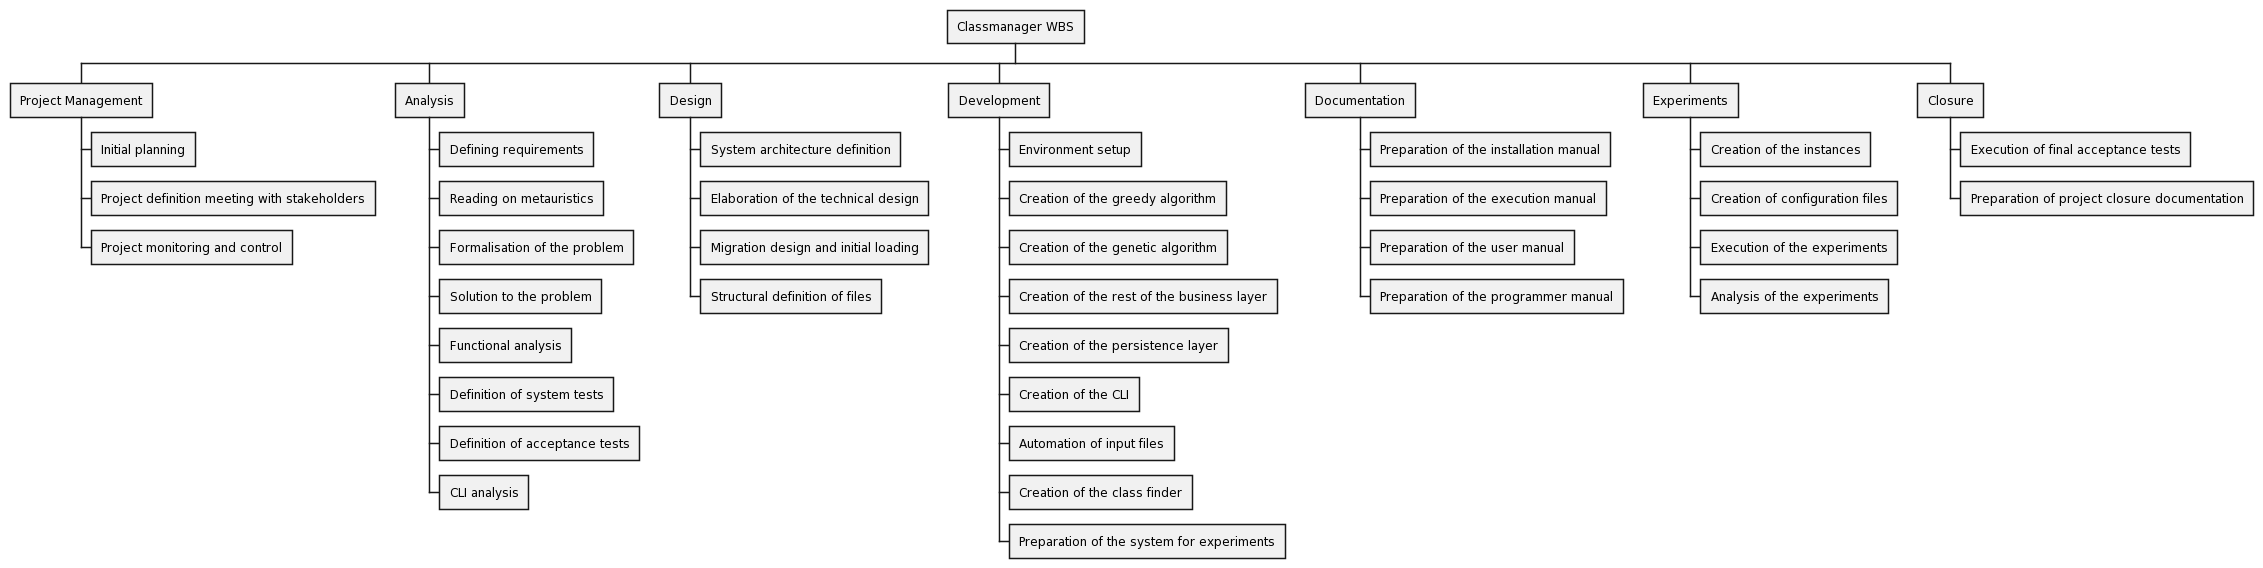
\includegraphics[scale=0.22]{wbs.png}
\end{figure}


\begin{figure}[H]
    \caption{Gantt chart}
  \centering
  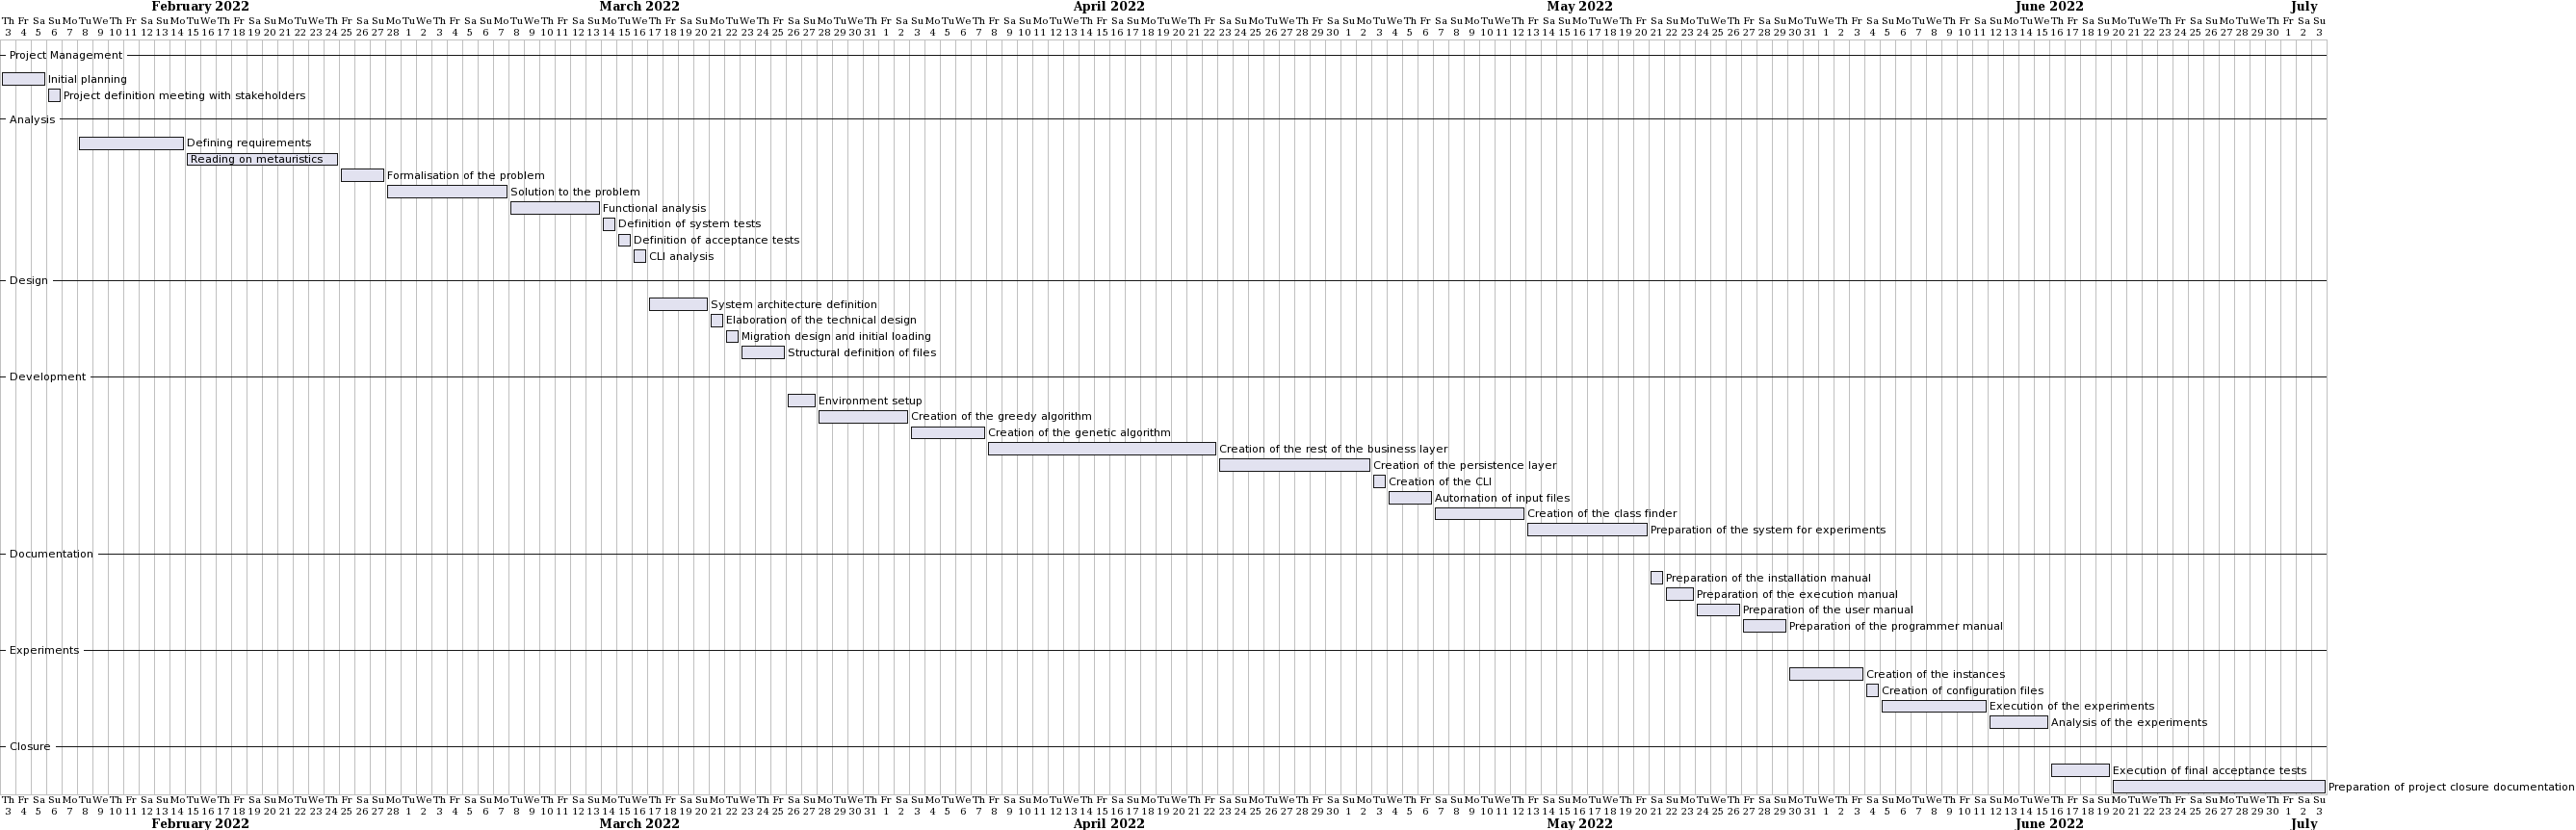
\includegraphics[scale=0.2, angle=90]{gantt.png}
\end{figure}


\subsection{Project Management}

\begin{itemize}
    \item \textbf{Initial planning}: Reading the project synopsis, first discussions with supervisors and establishing the project plan. 
    \item \textbf{Project definition meeting with stakeholders}: Requirements gathering meeting with the client, definition of objectives and scope of the project.
    \item \textbf{Project monitoring and control}: Regular meetings with supervisors and clients to discuss and review project status. 
\end{itemize}

\begin{figure}[H]
    \caption{Gantt chart: Project Management}
  \centering
  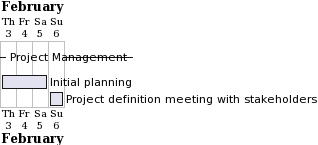
\includegraphics[scale=0.8]{gantt_01_project_management.png}
\end{figure}


\subsection{Analysis}

\begin{itemize}
    \item \textbf{Defining requirements}: Write down and review the requirements previously obtained in the meeting with the clients.
    \item \textbf{Reading on metaheuristics}: Reading diverse literature on greedy algorithms, genetic algorithms and metaheuristics. 
    \item \textbf{Formalisation of the problem}: Formal definition of the problem as an assignment problem, explaining its components and constraints.
    \item \textbf{Solution to the problem}: Theoretically elaborating the solution to the previously defined problem.
    \item \textbf{Functional analysis}: Analysis of use cases, functionality and other aspects of the software prototype.
    \item \textbf{Definition of system tests}: Tests on input files, configuration files and system functionality. 
    \item \textbf{Definition of acceptance tests}: Checking the quality of the results obtained by the system.
    \item \textbf{CLI analysis}: Study on how to run the utility and the format of its arguments. 
\end{itemize}

\begin{figure}[H]
    \caption{Gantt chart: Analysis}
  \centering
  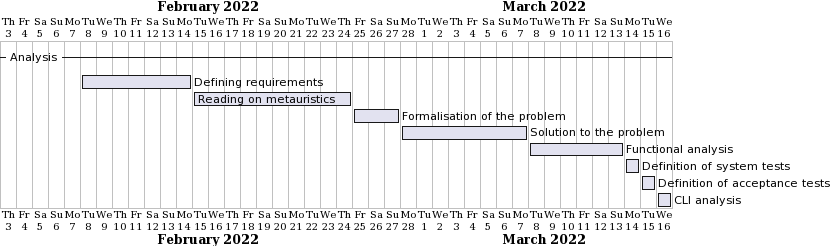
\includegraphics[scale=0.6]{gantt_02_analysis.png}
\end{figure}


\subsection{Design}

\begin{itemize}
    \item \textbf{System architecture definition}: Definition of subsystems, packages and the relationships between them.
    \item \textbf{Elaboration of the technical design}: Final class diagrams.
    \item \textbf{Migration design and initial loading}: Study on the conversion of planning and enrolment files into files with a format that can be processed by the system.
    \item \textbf{Structural definition of files}: Elaborating the final format of the input, output and configuration files. 
\end{itemize}

\begin{figure}[H]
    \caption{Gantt chart: Design}
  \centering
  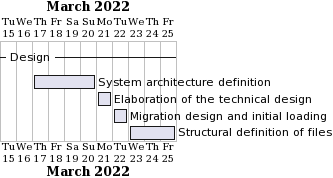
\includegraphics[scale=0.8]{gantt_03_design.png}
\end{figure}


\subsection{Development}

\begin{itemize}
    \item \textbf{Environment setup}: Creation of code and documentation repositories, configuration of text editors and tools to run and test the system.
    \item \textbf{Creation of the greedy algorithm}: Define the LCM, LFD, and the Greedy Algorithm components.
    \item \textbf{Creation of the genetic algorithm}: Define the operators of the Genetic Algorithm and its components.
    \item \textbf{Creation of the rest of the business layer}: Implement data infrastructure, log management, error handling and other business layer items. 
    \item \textbf{Creation of the persistence layer}: Develop DataAccess and file management. 
    \item \textbf{Creation of the CLI}: Utilities for all CLI content to be centralised in a single component.
    \item \textbf{Automation of input files}: Functionality of automating the files previously used by the School.
    \item \textbf{Creation of the class finder}: Functionality of searching classrooms with free time slots.
    \item \textbf{Preparations of the systems for experiments}: Adapt the system to make it easier to run many instances in parallel.
\end{itemize}

\begin{figure}[H]
    \caption{Gantt chart: Development}
  \centering
  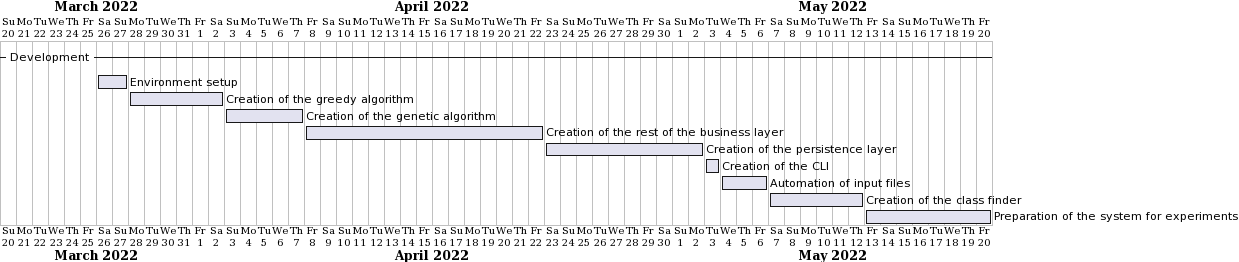
\includegraphics[scale=0.4]{gantt_04_development.png}
\end{figure}


\subsection{Documentation}

\begin{itemize}
    \item \textbf{Preparation of the installation manual}: Required dependencies and setup required to be able to run the application.
    \item \textbf{Preparation of the execution manual}: Available options for launching the software.
    \item \textbf{Preparation of the user manual}: Instructions on how to execute each functionality, explanation of how to interpret the output files and recommended configurations.
    \item \textbf{Preparation of the programmer manual}: Instructions on how to maintain the program, where to find the main parts of the code and how to interpret the log file.
\end{itemize}

\begin{figure}[H]
    \caption{Gantt chart: Documentation}
  \centering
  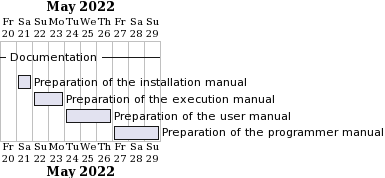
\includegraphics[scale=0.8]{gantt_05_documentation.png}
\end{figure}


\subsection{Experiments}

\begin{itemize}
    \item \textbf{Creation of the instances}: Instances are created based on actual data from past courses by using the automation functionality of the files used by the School.
    \item \textbf{Creation of configuration files}: Define the configuration files with the different combinations of values and parameters.
    \item \textbf{Execution of the experiments}: Execution of the experiments using a computer specialised in parallel runs.
    \item \textbf{Analysis of the experiments}: Analysis of the results and obtaining the best values in order to obtain the highest possible quality results.
\end{itemize}

\begin{figure}[H]
    \caption{Gantt chart: Experiments}
  \centering
  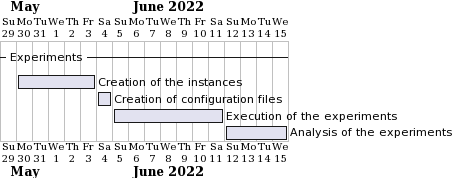
\includegraphics[scale=0.8]{gantt_06_experiments.png}
\end{figure}


\subsection{Closure}

\begin{itemize}
    \item \textbf{Execution of final acceptance tests}: Execution of tests to verify the quality of the results.
    \item \textbf{Preparation of the closure documentation}: Theoretical and technical project documentation.
\end{itemize}

\begin{figure}[H]
    \caption{Gantt chart: Closure}
  \centering
  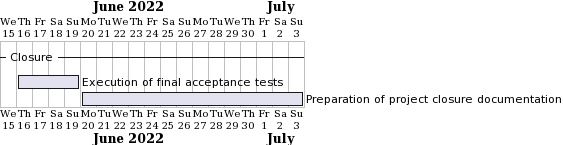
\includegraphics[scale=0.8]{gantt_07_closure.png}
\end{figure}



\section{Budget summary}

This section shows the internal and client buget summary of the project. They can be found in Figures \ref{fig-overview-internal-budget} and \ref{fig-overview-client-budget}. For the budget breakdown the reader is referred to Section \ref{section-budget}.


\begin{figure}[H]
    \caption{Internal budget summary}
    \label{fig-overview-internal-budget}
  \centering
  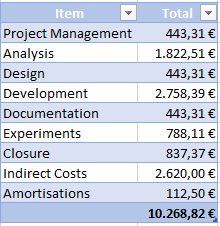
\includegraphics[scale=1]{budget_internal.PNG}
\end{figure}

\begin{figure}[H]
    \caption{Client budget summary}
    \label{fig-overview-client-budget}
  \centering
  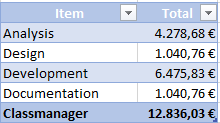
\includegraphics[scale=1]{budget_client.PNG}
\end{figure}



 

    \newpage
    \renewcommand{\documentname}{Analysis}

\chapter{Analysis}

In this second chapter of software engineering, we will present the analysis conducted on the system to be built, with a brief general definition of what is intended to be done, recapitulating what was previously discussed in the theoretical sections.

The system requirements, both functional and non-functional, are also introduced, followed by an identification of the internal components of the system, the subsystems. An outline of class design is shown, focusing on the relationships between classes and data, which continues with an analysis of the identified use cases and the user interface. The chapter ends with a discussion of the tests to be carried out on the system.



\section{System definition}

The prototype defined in this document consists of a command line application which receives a list of text files as input and, by processing them, can perform three operations. The first and main one is the calculation of all the assignments required for the semester, starting from scratch or by using a previous list of assignments generated by the system itself. The second operation consists of finding holes in the schedule, that is, to find free classrooms which comply with a set of constraints. This is useful for assigning a class to a specific event even if the exact time or day of such an event is not known and can only be guessed. The last operation is the automation of the creation of the input files, which is done by converting some other files previously used by the School into new files which the system is able to process.



\section{System requirements}

The functional and non-functional requirements of the system. The non-functional requirements include the technological, system manuals and response time requirements.

\subsection{Functional requirements}

\begin{description}

    \item \textbf{RCLI} The system must implement a command line interface (CLI).
        \begin{description}
            \item \textbf{RCLI1} The CLI must show information about the current process being executed.
            \item \textbf{RCLI2} The CLI must show information about the GA.
                \begin{description}
                    \item \textbf{RCLI2.1} About the parameters of the GA.
                    \item \textbf{RCLI2.2} About the generations of the GA.
                    \item \textbf{RCLI2.3} About the execution time of the GA.
                \end{description}
            \item \textbf{RCLI3} The CLI must show information about the result of the execution.
                \begin{description}
                    \item \textbf{RCLI3.1} If the system terminated successfully.
                    \item \textbf{RCLI3.2} If the system terminated with errors, they will be also notified to the user.
                \end{description}
        \end{description}

    \item \textbf{RInput1} The system must receive the required data as input.
        \begin{description}
            \item \textbf{RInput1.1} The system must receive as input the classrooms of the School.
            \item \textbf{RInput1.2} The system must receive as input the groups of the semester.
            \item \textbf{RInput1.3} The system must receive as input the schedule of the groups.
            \item \textbf{RInput1.4} The system must receive as input the weeks in which the groups have classes.
            \item \textbf{RInput1.5} The system must receive as input the subjects of the semester.
            \item \textbf{RInput1.6} The system must receive as input the queries with the constraints for finding free classrooms in the schedule.
            \item \textbf{RInput1.7} The system must receive as input the previously used files for the automation of the system input files.
        \end{description}

    \item \textbf{RInput2} The system might receive optional data as input.
        \begin{description}
            \item \textbf{RInput2.1} The system might receive as input a total or partial list of assignments.
            \item \textbf{RInput2.2} The system might receive as input a list of classroom preferences.
            \item \textbf{RInput2.3} The system might receive as input a list of classroom restrictions.
        \end{description}

    \item \textbf{RInput3} The system must receive the required configuration files as input.
        \begin{description}
            \item \textbf{RInput3.1} The configuration files can be split into any number of files.
            \item \textbf{RInput3.2} The configuration files must include the information required by each functionality.
        \end{description}

    \item \textbf{RConf} The system must be configured by plain text files.
        \begin{description}
            \item \textbf{RConf1} System configuration must allow the user to control the parameters of the GA.
            \item \textbf{RConf2} System configuration must allow the user to specify the paths of the input files.
            \item \textbf{RConf3} System configuration must allow the user to specify the folder paths for the output files.
        \end{description}

    \item \textbf{RAssign} The system must perform the assignments by using AI algorithms.
        \begin{description}
            \item \textbf{RAssign1} The assignments should prioritise that Spanish and English groups go to different classes. 
            \item \textbf{RAssign2} The assignments may start from an initial set of assignments which must remain the same.
            \item \textbf{RAssign3} The assignments must maximize the number of groups of the same name and course assigned to the same theory classroom.
            \item \textbf{RAssign4} The assignments must maximize the number of groups of the same subject assigned to the same laboratory.
            \item \textbf{RAssign5} The assignments must leave a number of free laboratories in each time slot.
            \item \textbf{RAssign6} The assignments should prioritise that a laboratory does not end up with a large number of unused computers.
        \end{description}

    \item \textbf{RClassFinder} The system must be able to find free classrooms for an event given some constraints.
        \begin{description}
            \item \textbf{RClassFinder1} The constraints must include the date range for the search.
            \item \textbf{RClassFinder2} The constraints must include the range of hours for the search. 
            \item \textbf{RClassFinder3} The constraints must include the duration of the event (in hours) for the search.
            \item \textbf{RClassFinder4} The constraints must include the number of attendants to the event. 
            \item \textbf{RClassFinder5} The constraints must include the type of classroom to hold the event in. 
            \item \textbf{RClassFinder6} The constraints must include the maximum number of results to obtain. 
        \end{description}

    \item \textbf{RAutomation} The system must be able to automate the creation of the input files.
        \begin{description}
            \item \textbf{RAutomation1} The system must receive the planning for the semester.
            \item \textbf{RAutomation2} The system must receive the number of enrolled students for each group.
        \end{description}

    \item \textbf{RLog} The system must keep a log of its operations.
        \begin{description}
            \item \textbf{RLog1} The log must indicate the date and time of every record.
            \item \textbf{RLog2} The log must indicate the log level of every record.
            \item \textbf{RLog3} The log must record the complete information of encountered errors.
            \item \textbf{RLog4} The log must record basic information of the flow of the application.
        \end{description}

\end{description}


\subsection{Non-Functional requirements}

\begin{description}

    \item \textbf{RTech} The system requires a specific setup to be executed.
        \begin{description}
            \item \textbf{RTech1} The system requires Java 8 to be installed in the computer which executes it.
            \item \textbf{RTech2} The system requires that the folders where the input files are located have sufficient permissions for the system to be able to read these files.
        \end{description}

    \item \textbf{RMan} The system manuals must provide the readers with appropriate information for carrying out their tasks.  
        \begin{description}
            \item \textbf{RMan1} The installation manual must explain the setup needed before the execution of the program.
                \begin{description}
                    \item \textbf{RMan1.1} It is aimed both at the user and the developers of the application.
                \end{description}
            \item \textbf{RMan2} The execution manual must explain the syntax for executing each functionality of the system.
                \begin{description}
                    \item \textbf{RMan2.1} It is aimed both at the user and the developers of the application.
                \end{description}
            \item \textbf{RMan3} The user manual must explain all the functionality of the system.
                \begin{description}
                    \item \textbf{RMan3.1} It is aimed at the user of the application.
                    \item \textbf{RMan3.2} It must provide examples of usage with step by step instructions. 
                \end{description}
            \item \textbf{RMan4} The programmer manual must briefly explain the structure of the code and its components.
                \begin{description}
                    \item \textbf{RMan4.1} It is aimed at the developers and maintainers of the application.
                    \item \textbf{RMan4.2} It must provide examples of possible changes with some directions to implement them. 
                    \item \textbf{RMan4.3} It must provide an explanation on how to interpret the log of the application. 
                \end{description}
        \end{description}

    \item \textbf{RResponse} The system must perform the assignments of a semester in less than a day.
        \begin{description}
            \item \textbf{RResponse1} The assignments must have the expected quality. An assignment is said to be of quality if it meets all hard and as many soft constraints as possible.
        \end{description}

\end{description}



\section{Subsystem mapping}

In order to better understand the system, a study has been carried out on the subsystems that make up the system. The following subsystems have been identified:

\begin{itemize}

    \item \textbf{Algorithm subsystem:} Contains the greedy and genetic algorithms, as well as their operators and procedures.

    \item \textbf{Classfinder subsystem:} Contains functionality relating to the search for free classes in a time and schedule range.

    \item \textbf{Configuration subsystem:} Parses configuration files and keeps them in memory.

    \item \textbf{ErrorHandler subsystem:} It addresses the errors encountered and differentiates the expected from the unexpected.

    \item \textbf{Log subsystem:} It is in charge of creating and updating the system log.

    \item \textbf{Problem domain subsystem:} Defines the abstractions of the problem in the form of object types.

    \item \textbf{Central subsystem:} In charge of connecting the other subsystems to carry out the different functionalities of the system.

    \item \textbf{Persistence subsystem:} Responsible for parsing input files and constructing output files.

    \item \textbf{CLI subsystem:} Handles all text output to the console.

\end{itemize}




\section{Preliminary class diagram}


\begin{figure}[H]
    \caption{Preliminary class diagram}
  \centering
  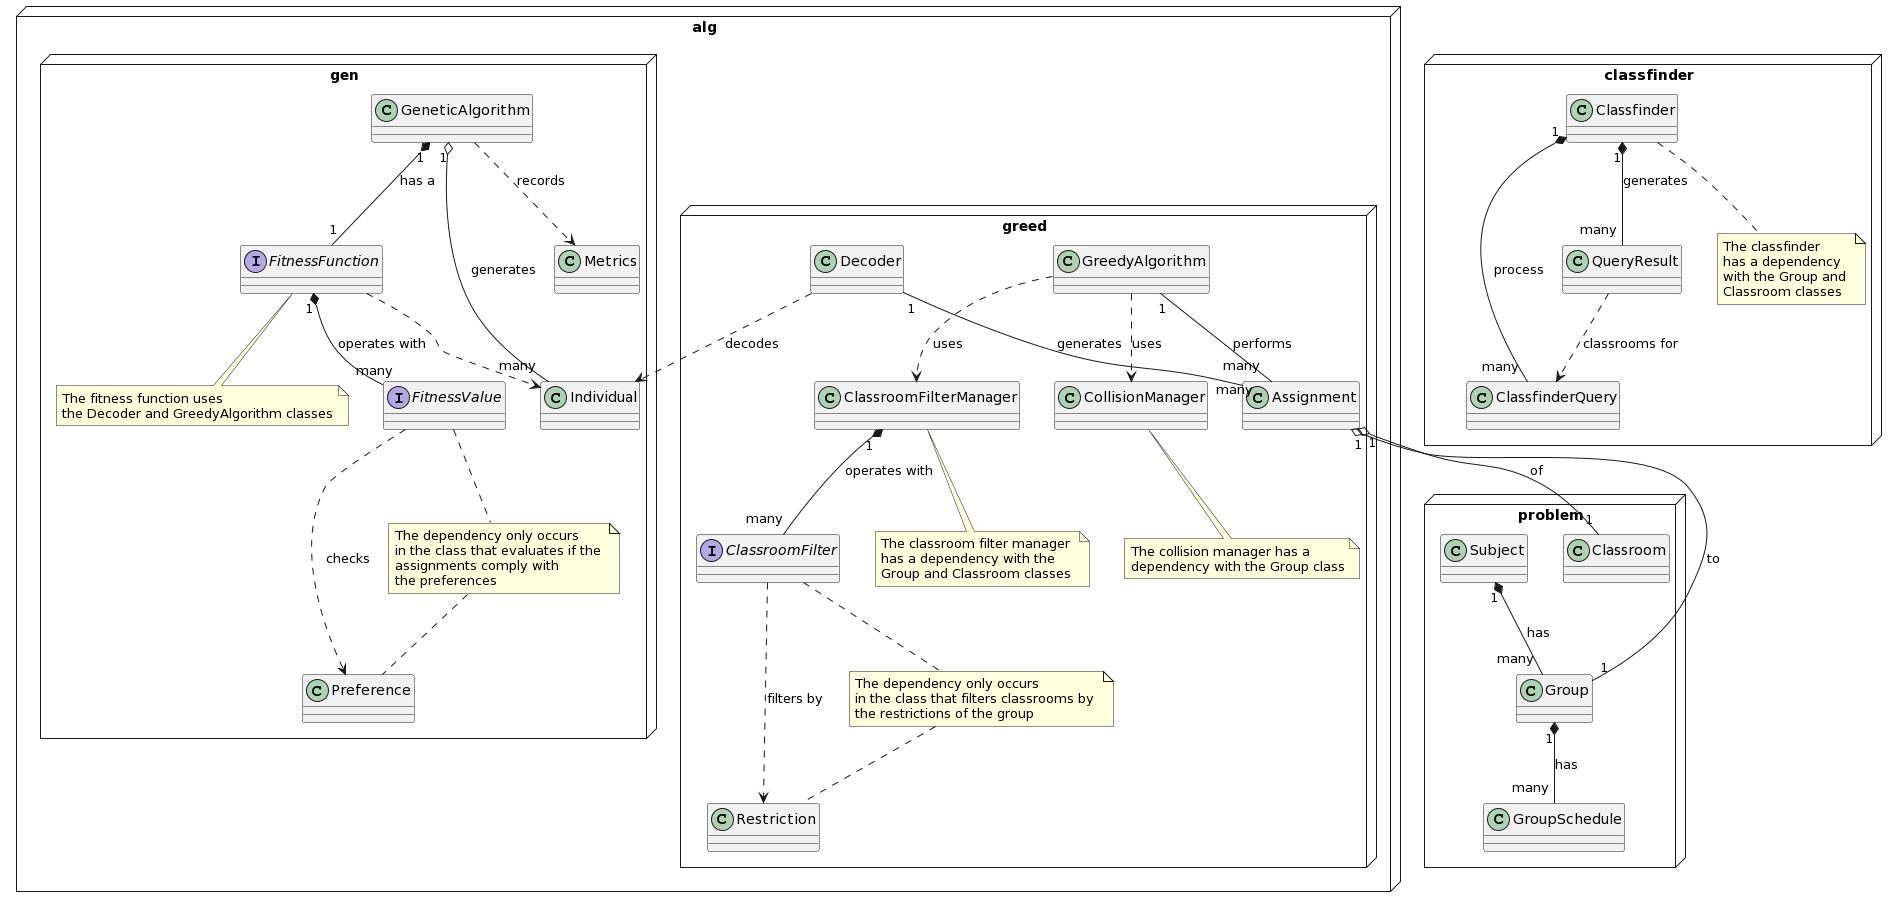
\includegraphics[scale=0.25]{initial_class_diagram_uml.png}
\end{figure}

Some notes on the previously shown class draft. It only contains classes from the business layer, because it is the most important part of the prototype.

The \textit{alg} package contains all classes related to the genetic and greedy algorithms. They are both interconnected by means of the fitness function of the GA, which uses the Decoder to get the assignments in the order specified by an individual and then calls the greedy algorithm with such a list of assignments. In the case of the greedy algorithm, some of its components, like the ClassroomFilterManager (which models the LFD) and the CollisionManager (which models the LCM) have a dependency with some classes of the problem domain package. That is also the case for the Assignment class, which represents an assignment of a classroom to a group.

The \textit{classfinder} package is a little more isolated than the alg package, but nevertheless has dependencies with some classes of the problem domain.

Finally, the \textit{problem} package models the problem domain, and contains the information of the abstracted models of the School and its environment. It is a key package not only for the different packages of the business layer, but also for the persistence layer, which depends on it for implementing the DataAccess to each abstraction.


\section{Analysis of use cases}

This section presents the analysis of the use cases of the system. Three use cases have been identified, each one reflecting a main functionality of the prototype. Therefore we have a use case for the assignment of classes to groups, the search for free classes by means of specific queries and the automatic generation of the system input files.

\begin{figure}[H]
    \caption{Use cases}
  \centering
  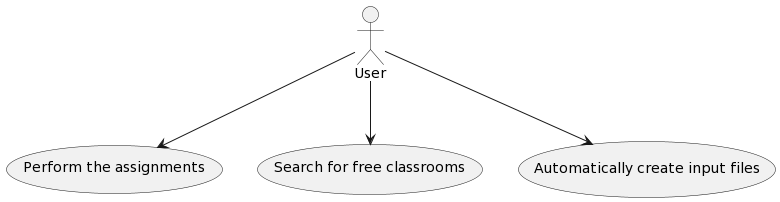
\includegraphics[scale=0.5]{use_cases_uml.png}
\end{figure}

For each use case, a table with information about the use case is presented. These tables contain the preconditions for the use case, the postconditions reached after its execution, a description of its steps, and a section with other variants of the use case. These tables are followed by a sequence and an activity diagrams, which will show the flow of the use case in a more visual way.

\subsection{Perform the assignments}

\begin{table}[H]
    \centering
    \caption{Use case description: Perform the assignments}
    \label{uc-table-assignments}
    \begin{tabular}{|p{4cm}|p{12cm}|}
        \hline
        \multicolumn{2}{|c|}{\textbf{PERFORM THE ASSIGNMENTS}} \\
        \hline
        \rowcolor{blue!10}
        \textbf{PRECONDITIONS} & \textit{The configuration files containing information about the GA and the input files need to be correctly formatted and must include the required data. Moreover, the input files with the classrooms, subjects, groups, group schedules, group academic weeks, restrictions, preferences and initial assignments must be correctly formatted.} \\
        \rowcolor{blue!30}
        \textbf{POSTCONDITIONS} & \textit{A text file with a report on the calculated assignments is generated. Also, a csv file with the assignments in the required format and a text file per classroom indicating its schedule in a timetable format are also written.} \\
        \rowcolor{blue!10}
        \textbf{DESCRIPTION} & 
        \textit{\begin{itemize}
                \item The user executes the program with the option flag signaling the calculation of the assignments and the path to the required configuration files.
                \item The system parses the configuration files. 
                \item The system parses the required and optional files indicated in the configuration files, as well as the GA parameters.
                \item The system executes the algorithms.
                \item The system outputs the best individual's information into a report text file, a csv file with the assignments and a text file for each classroom with its timetable.
            \end{itemize}
        } \\
        \rowcolor{blue!30}
        \textbf{SECONDARY SCENARIOS (VARIANTS)} & 
        \textbf{Variant 1. Errors on parsing.} If the system encounters any errors while parsing the input files, it will notify the user and store the information about such errors in the log file.
        \textbf{Variant 2. Not enough permissions.} If the system cannot read from or write into a folder because of insufficient permissions, it will notify the user and store the information about the error in the log file.
        \\
        \hline
    \end{tabular}
\end{table}


\begin{figure}[H]
    \caption{Sequence diagram: Perform the assignments}
  \centering
  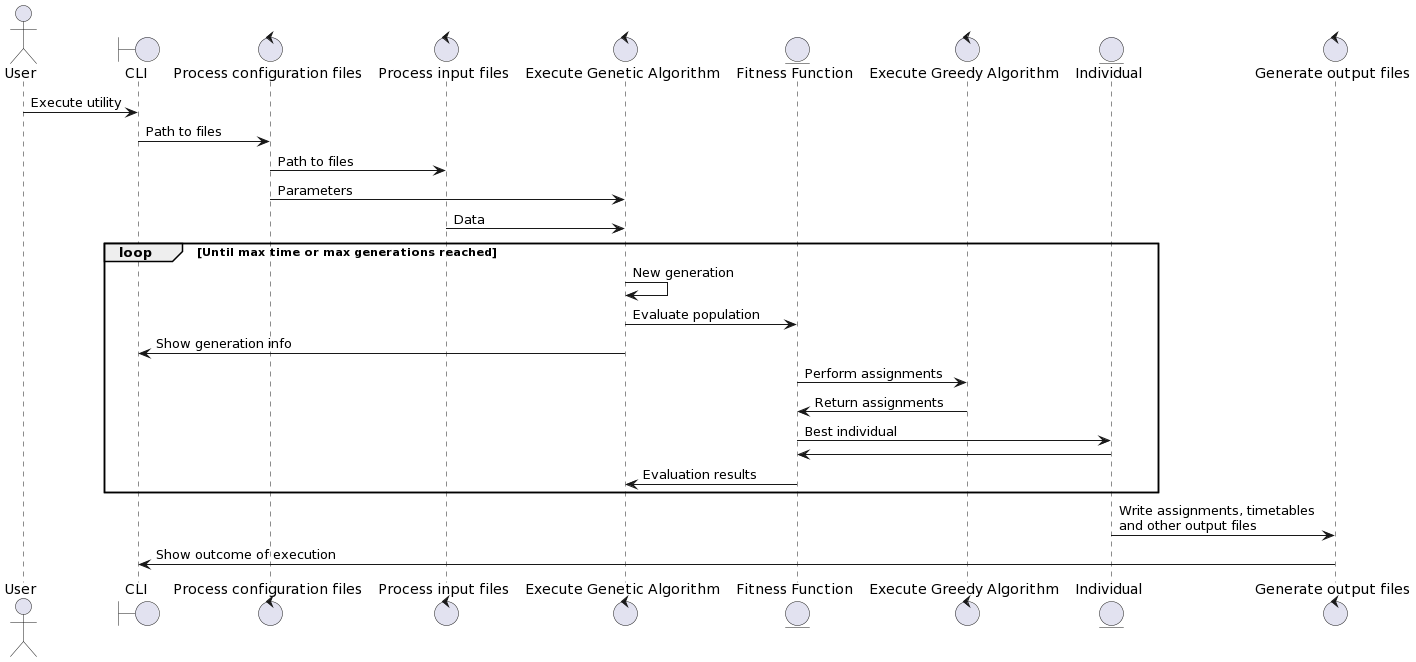
\includegraphics[scale=0.3]{uc_assignments_sequence_uml.png}
\end{figure}


\begin{figure}[H]
    \caption{Activity diagram: Perform the assignments}
  \centering
  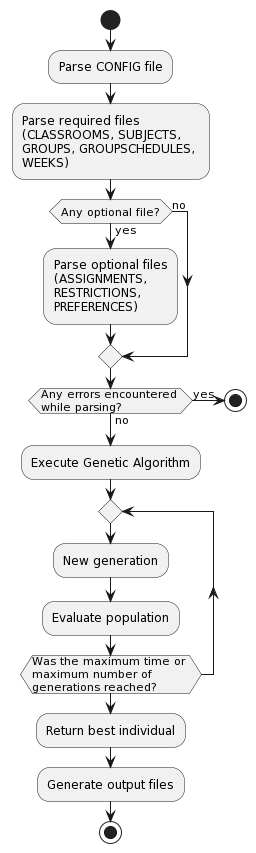
\includegraphics[scale=0.45]{uc_assignments_activity_uml.png}
\end{figure}




\subsection{Search for free classrooms}

\begin{table}[H]
    \centering
    \caption{Use case description: Search for free classrooms}
    \begin{tabular}{|p{4cm}|p{12cm}|}
        \hline
        \multicolumn{2}{|c|}{\textbf{SEARCH FOR FREE CLASSROOMS}} \\
        \hline
        \rowcolor{blue!10}
        \textbf{PRECONDITIONS} & \textit{The configuration files containing information about the input files needs to be correctly formatted and must include the required data. Moreover, the input files with the classrooms, subjects, groups, group schedules, group academic weeks, assignments and queries must be correctly formatted.} \\
        \rowcolor{blue!30}
        \textbf{POSTCONDITIONS} & \textit{A text file with the query results is generated.} \\
        \rowcolor{blue!10}
        \textbf{DESCRIPTION} & 
        \textit{\begin{itemize}
                \item The user executes the program with the option flag signaling the execution of the queries for finding free classrooms and the path to the required configuration files.
                \item The system parses the configuration files. 
                \item The system parses the required files indicated in the configuration files.
                \item The system executes the queries.
                \item The system outputs the result of all queries into a text file.
            \end{itemize}
        }\\
        \rowcolor{blue!30}
        \textbf{SECONDARY SCENARIOS (VARIANTS)} & \textit{Same as in Table \ref{uc-table-assignments}} \\
        \hline
    \end{tabular}
\end{table}


\begin{figure}[H]
    \caption{Sequence diagram: Search for free classrooms}
  \centering
  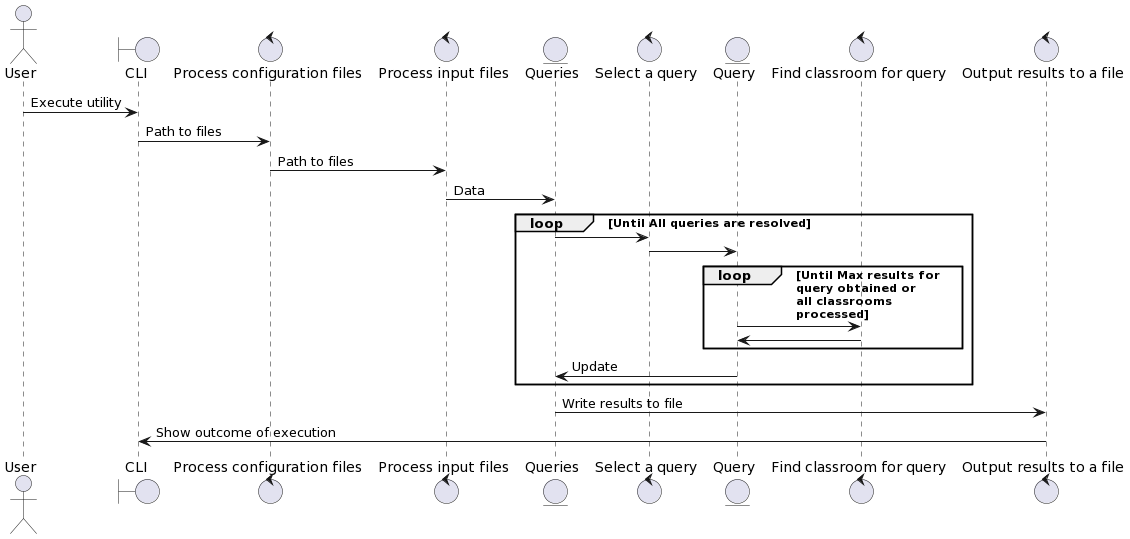
\includegraphics[scale=0.4]{uc_classfinder_sequence_uml.png}
\end{figure}


\begin{figure}[H]
    \caption{Activity diagram: Search for free classrooms}
  \centering
  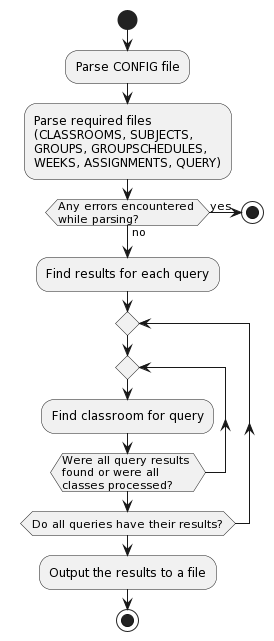
\includegraphics[scale=0.5]{uc_classfinder_activity_uml.png}
\end{figure}



\subsection{Automatically create input files}

\begin{table}[H]
    \centering
    \caption{Use case description: Automatically create input files}
    \begin{tabular}{|p{4cm}|p{12cm}|}
        \hline
        \multicolumn{2}{|c|}{\textbf{AUTOMATICALLY CREATE INPUT FILES}} \\
        \hline
        \rowcolor{blue!10}
        \textbf{PRECONDITIONS} & \textit{The configuration files containing information about the input files needs to be correctly formatted and must include the required data. Moreover, the input files with the planning for the semester and the number of enrolled students for each group must be correctly formatted.} \\
        \rowcolor{blue!30}
        \textbf{POSTCONDITIONS} & \textit{The files with the data of the subjects, groups, group schedules and group academic weeks are generated.} \\
        \rowcolor{blue!10}
        \textbf{DESCRIPTION} & 
        \textit{\begin{itemize}
                \item The user executes the program with the option flag signaling the generation of the input files and the path to the required configuration files.
                \item The system parses the configuration files. 
                \item The system parses the required files indicated in the configuration files.
                \item The system transforms the input files into the required format.
                \item The system outputs the result of each transformation in their own files.
            \end{itemize}
        }\\
        \rowcolor{blue!30}
        \textbf{SECONDARY SCENARIOS (VARIANTS)} & \textit{Same as in Table \ref{uc-table-assignments}} \\
        \hline
    \end{tabular}
\end{table}


\begin{figure}[H]
    \caption{Sequence diagram: Automatically create input files}
  \centering
  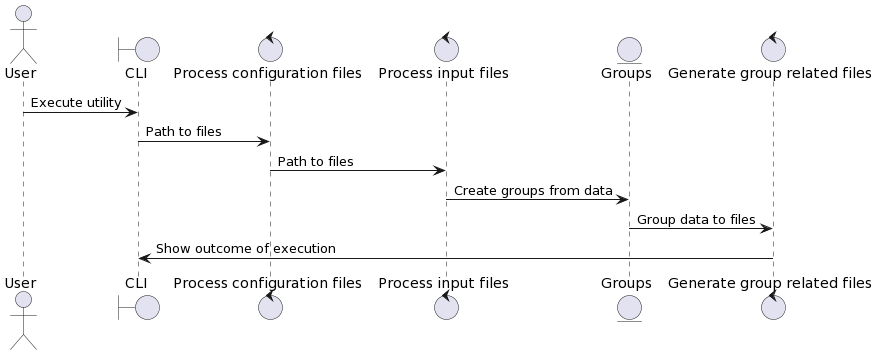
\includegraphics[scale=0.4]{uc_automation_sequence_uml.png}
\end{figure}


\begin{figure}[H]
    \caption{Activity diagram: Automatically create input files}
  \centering
  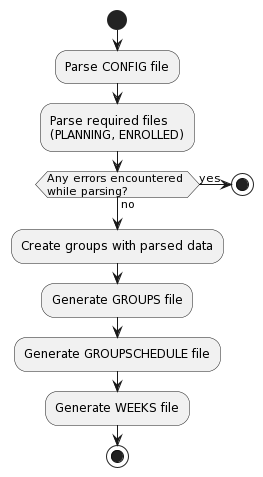
\includegraphics[scale=0.6]{uc_automation_activity_uml.png}
\end{figure}




\section{Analysis of user interfaces}

The prototype will have a Command Line Interface (CLI). The only interaction with the user occurs when they are calling the utility in the shell, indicating the option they want the prototype to execute and the necessary configuration files. As we explained before in the document, there are three main options for calling the prototype. One for performing the assignments, the second for finding free classrooms and the third for automating the creation of the input files.

Once the execution starts, the CLI will show relevant information to the user about the currently running processes (name and status). In the case of the GA execution, the selected parameters will be listed, as well as data on the results of each generation. The amount of information shown in the CLI about the GA can be controlled by the user through the configuration files. 



\section{Test plan specification}

Testing will focus on the parsing phase and the quality of the solutions obtained. In order to verify that both areas operate as expected, a battery of functional tests and an experimentation with various scenarios and instances will be carried out. Further details of the conducted experimentation are given in its own section (see Section \ref{experimental-results}), here we will focus on the test suite.


\begin{table}[H]
    \centering
    \caption{Test suite for UC: Perform the assignments}
    \label{uc-table-assignments}
    \begin{tabular}{|p{4cm}|p{8cm}|}
        \hline
        \multicolumn{2}{|c|}{\textbf{PERFORM THE ASSIGNMENTS}} \\
        \hline
        \textbf{Test} & \textbf{Expected result} \\
        \rowcolor{blue!30}
        No optional files & The assignment process will start from scratch and no restrictions or preferences are to be considered. \\
        \rowcolor{blue!10}
        Preferences & The assignment process will start from scratch and no restrictions are to be considered. Positive and negative preferences will be evaluated as soft constraints. \\
        \rowcolor{blue!30}
        Restrictions & The assignment process will start from scratch and no preferences are to be considered. Positive and negative restrictions will be evaluated as hard constraints. \\
        \rowcolor{blue!10}
        Partial assignments & The assignment process will start from the initial assignments and no preferences or restrictions are to be considered. The initial assignments will remain as they were once the allocation process is completed. \\
        \rowcolor{blue!30}
        All optional files & The assignment process will start from the initial assignments and the restrictions and preferences will be taken into account. \\
        \rowcolor{blue!10}
        Incorrect config format & The system will notify the error to the user. \\
        \rowcolor{blue!30}
        Incorrect input file format & The system will notify the error to the user. \\
        \rowcolor{blue!10}
        Incorrect input data & The system will notify the error to the user \\
        \hline
    \end{tabular}
\end{table}


\begin{table}[H]
    \centering
    \caption{Test suite for UC: Search for free classrooms}
    \label{uc-table-assignments}
    \begin{tabular}{|p{4cm}|p{8cm}|}
        \hline
        \multicolumn{2}{|c|}{\textbf{SEARCH FOR FREE CLASSROOMS}} \\
        \hline
        \textbf{Test} & \textbf{Expected result} \\
        \rowcolor{blue!30}
        Theory query & The system will look for theory classes that meet the requirements of the query. \\
        \rowcolor{blue!10}
        Lab query & The system will look for laboratories that meet the requirements of the query. \\
        \rowcolor{blue!30}
        Theory and lab query & The system will look for theory classes for one request and laboratories for the other. Each search must meet the requirements of its associated query. \\
        \rowcolor{blue!10}
        Incorrect config format & The system will notify the error to the user. \\
        \rowcolor{blue!30}
        Incorrect input file format & The system will notify the error to the user. \\
        \rowcolor{blue!10}
        Incorrect input data & The system will notify the error to the user \\
        \hline
    \end{tabular}
\end{table}


\begin{table}[H]
    \centering
    \caption{Test suite for UC: Automatically create input files}
    \label{uc-table-assignments}
    \begin{tabular}{|p{4cm}|p{8cm}|}
        \hline
        \multicolumn{2}{|c|}{\textbf{AUTOMATICALLY CREATE INPUT FILES}} \\
        \hline
        \textbf{Test} & \textbf{Expected result} \\
        \rowcolor{blue!30}
        Automation & The system will generate the input files necessary for the GA execution. \\
        \rowcolor{blue!10}
        Incorrect config format & The system will notify the error to the user. \\
        \rowcolor{blue!30}
        Incorrect input file format & The system will notify the error to the user. \\
        \rowcolor{blue!10}
        Incorrect input data & The system will notify the error to the user \\
        \hline
    \end{tabular}
\end{table}

 

    \newpage
    \renewcommand{\documentname}{System design}

\chapter{System design}


Until now we have seen a theoretical view of the algorithms, with some pseudocode, and an abstracted technical view of the system with the analysis discussed in the previous chapter. This chapter presents to the reader, with the help of different diagrams, a more technical side to the prototype in which the actual code of the utility will be based. The software architecture, the detailed class diagram and the format of the files used by the system follow.


\section{System architecture}

The architecture of the system is laid out in two diagrams, the component diagram, which models the relationship between the subsystems and their interfaces; and the package diagram, which shows the logical layout of the code.

The component diagram is depicted below (see Figure \ref{compo-diagram}).


\begin{figure}[H]
    \caption{Components diagram}
    \label{compo-diagram}
  \centering
  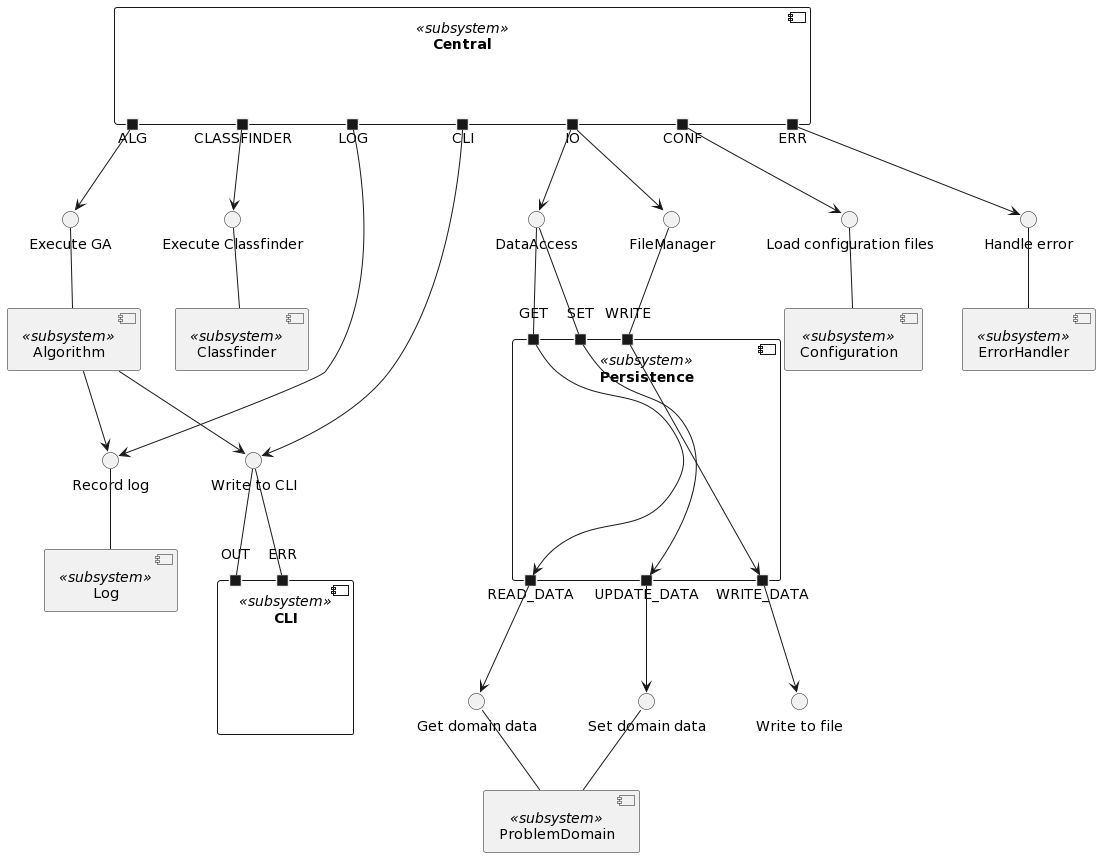
\includegraphics[scale=0.4]{components_diagram_uml.png}
\end{figure}

It can be seen that the central subsystem is responsible for connecting the major subsystems with each other, especially those belonging to the different code layers. Only the central subsystem and the algorithm subsystem have direct access to the log and the CLI.

The relationship between the persistence layer and the problem domain subsystem is due to the fact that it is the former that creates the data for the latter, and once the central subsystem receives this data, it is responsible for providing said data to the different components that require it.

The package diagram follows (see Figure \ref{pack-diagram}).

\begin{figure}[H]
    \caption{Packages diagram}
    \label{pack-diagram}
  \centering
  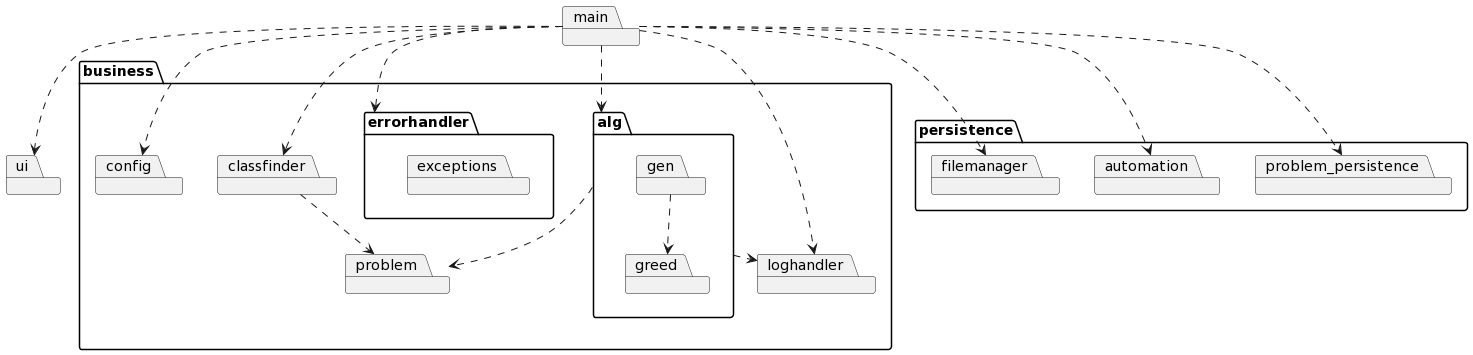
\includegraphics[scale=0.3]{packages_diagram_uml.png}
\end{figure}

What is noteworthy of this diagram is the appearance of new elements that the initial class diagram did not have. For example, the error handler contains both its logic and the definition of the prototype's own exceptions. The log handler contains a reference to the internal Java log logic, and acts as a wrapper that facilitates communication with other modules. Finally, the persistence layer has three main packages: the file manager, in charge of writing and reading files; the automation functionality of the files from the School to our files; and finally the DataAccess to the files of the domain.




\section{Class design}

This section presents the different class diagrams that make up the whole system, without showing trivial details and without repeating elements with similar layouts, in order to enhance readability.


\begin{figure}[H]
    \caption{Class diagram: Alg package}
  \centering
  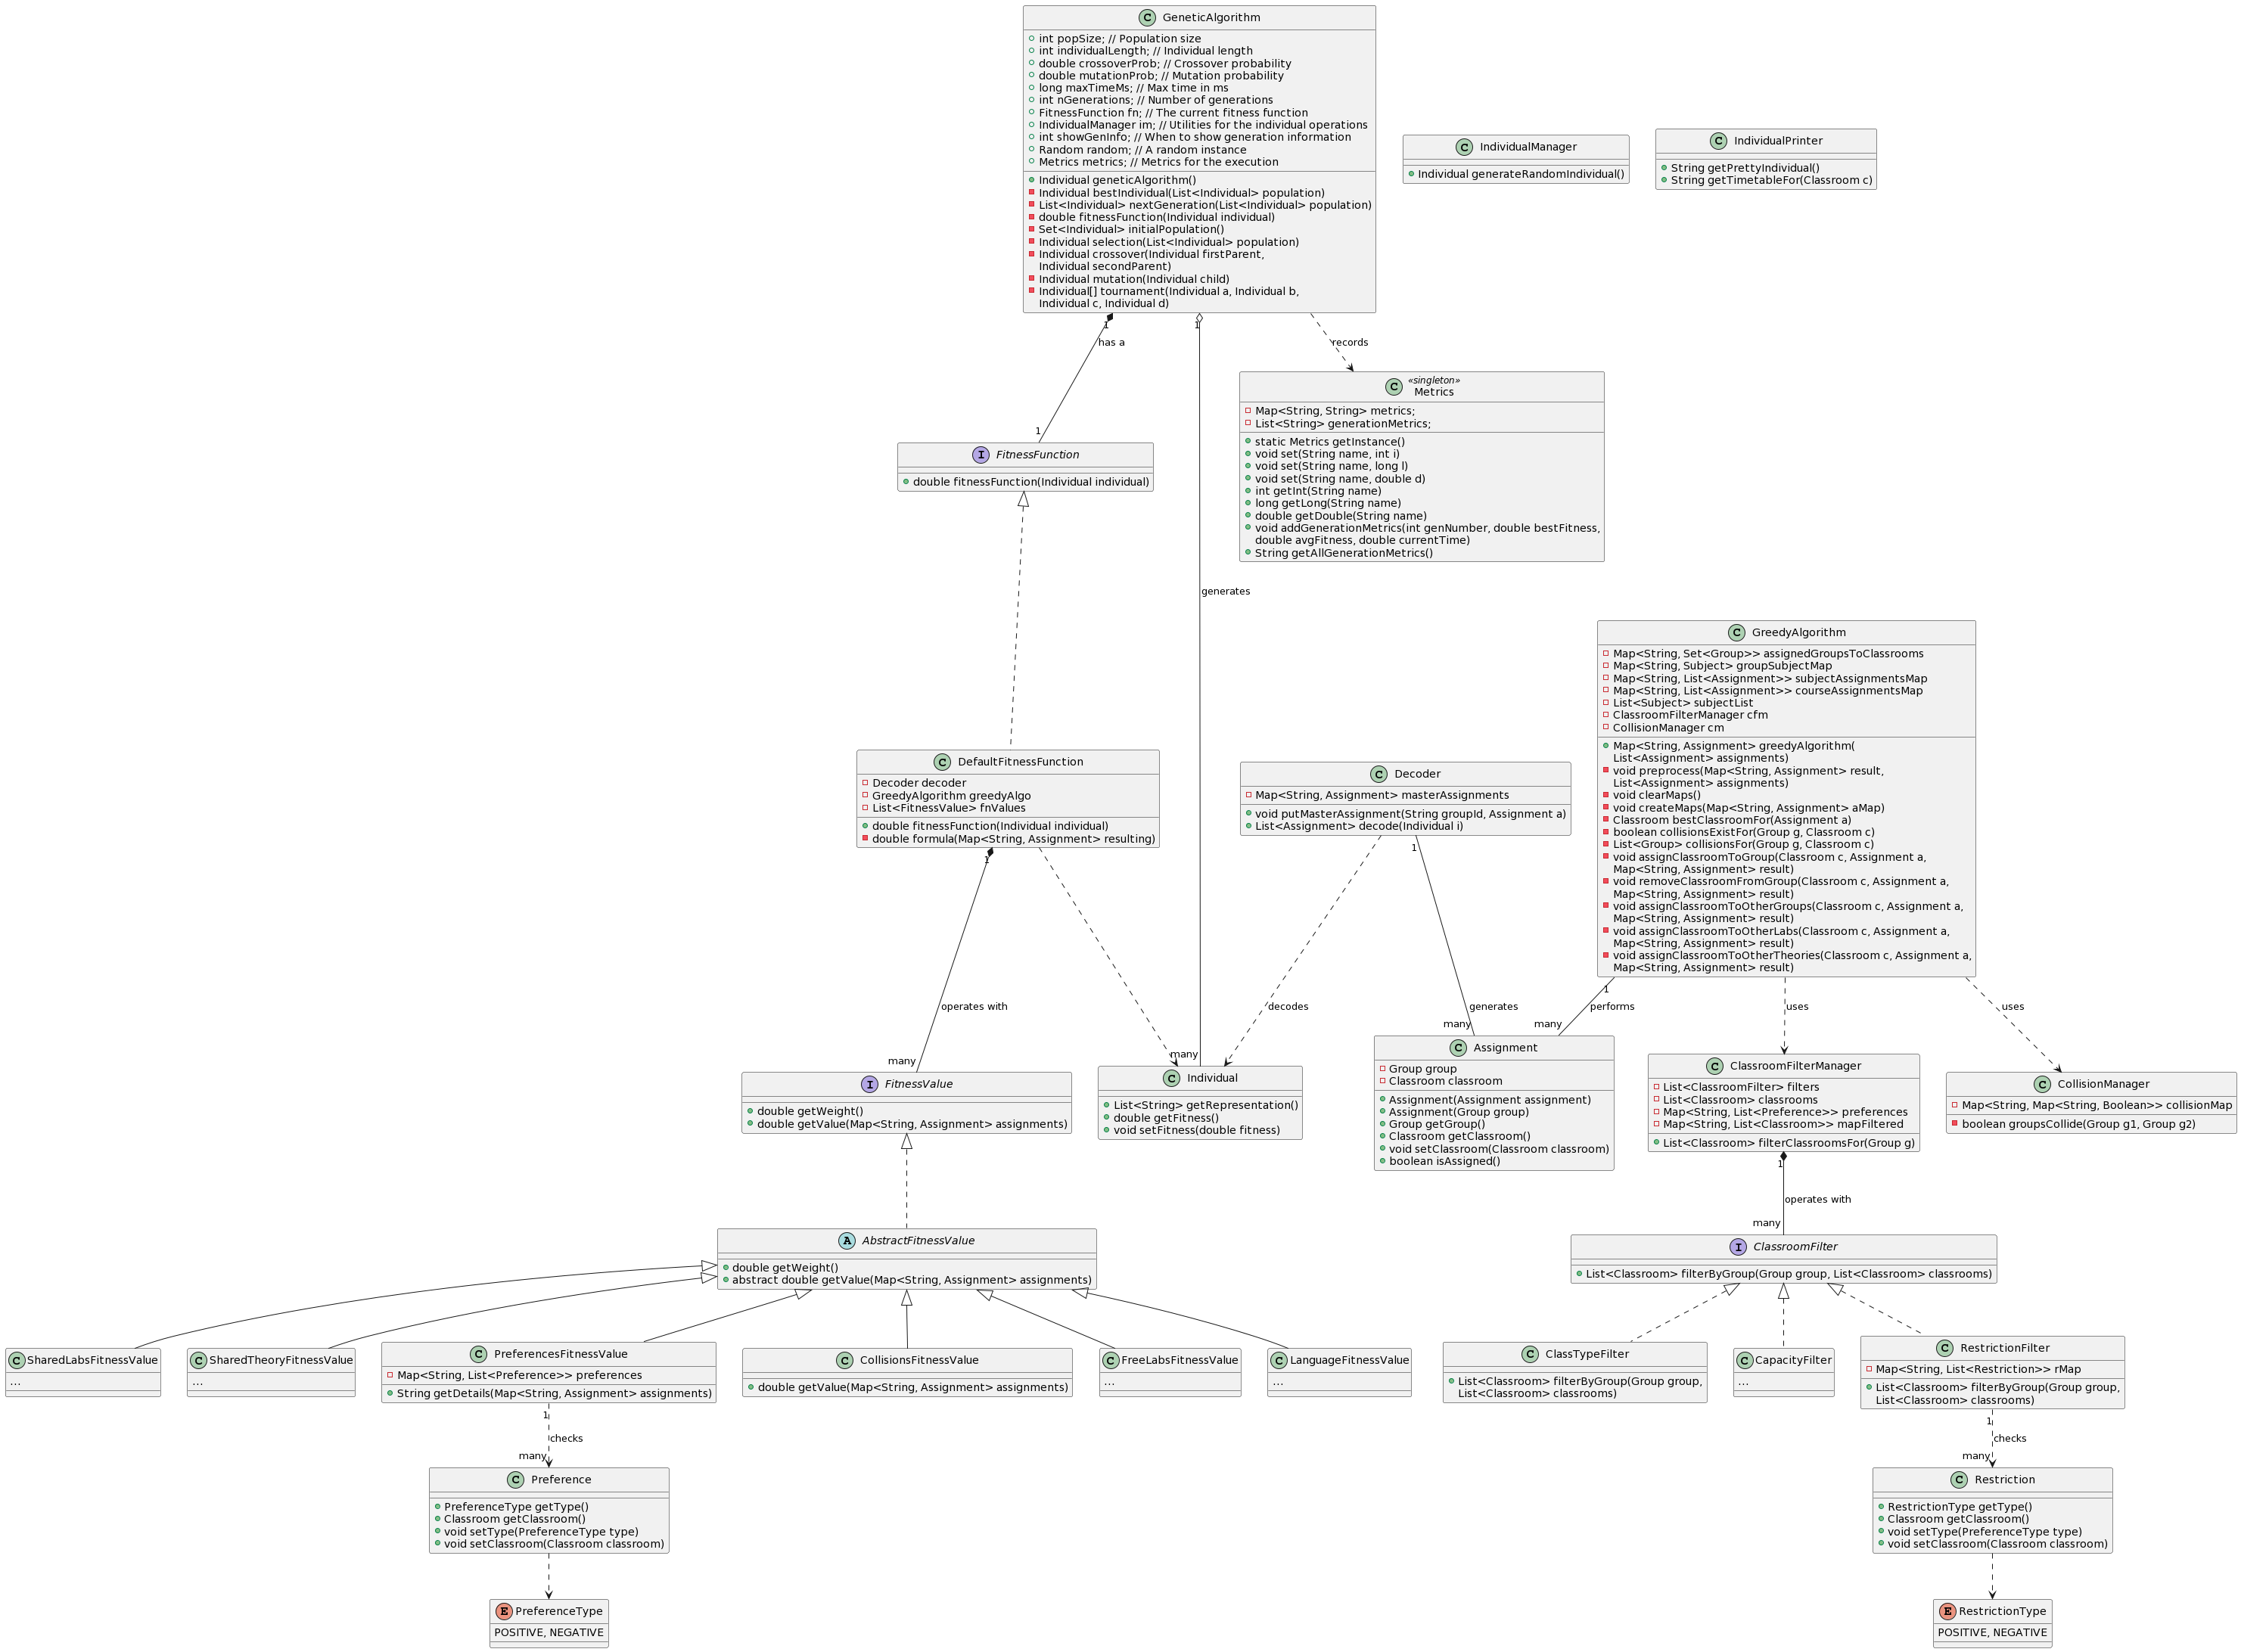
\includegraphics[scale=0.15]{final_alg_class_diagram_uml.png}
\end{figure}

\begin{figure}[H]
    \caption{Class diagram: Alg package (Greedy algorithm)}
  \centering
  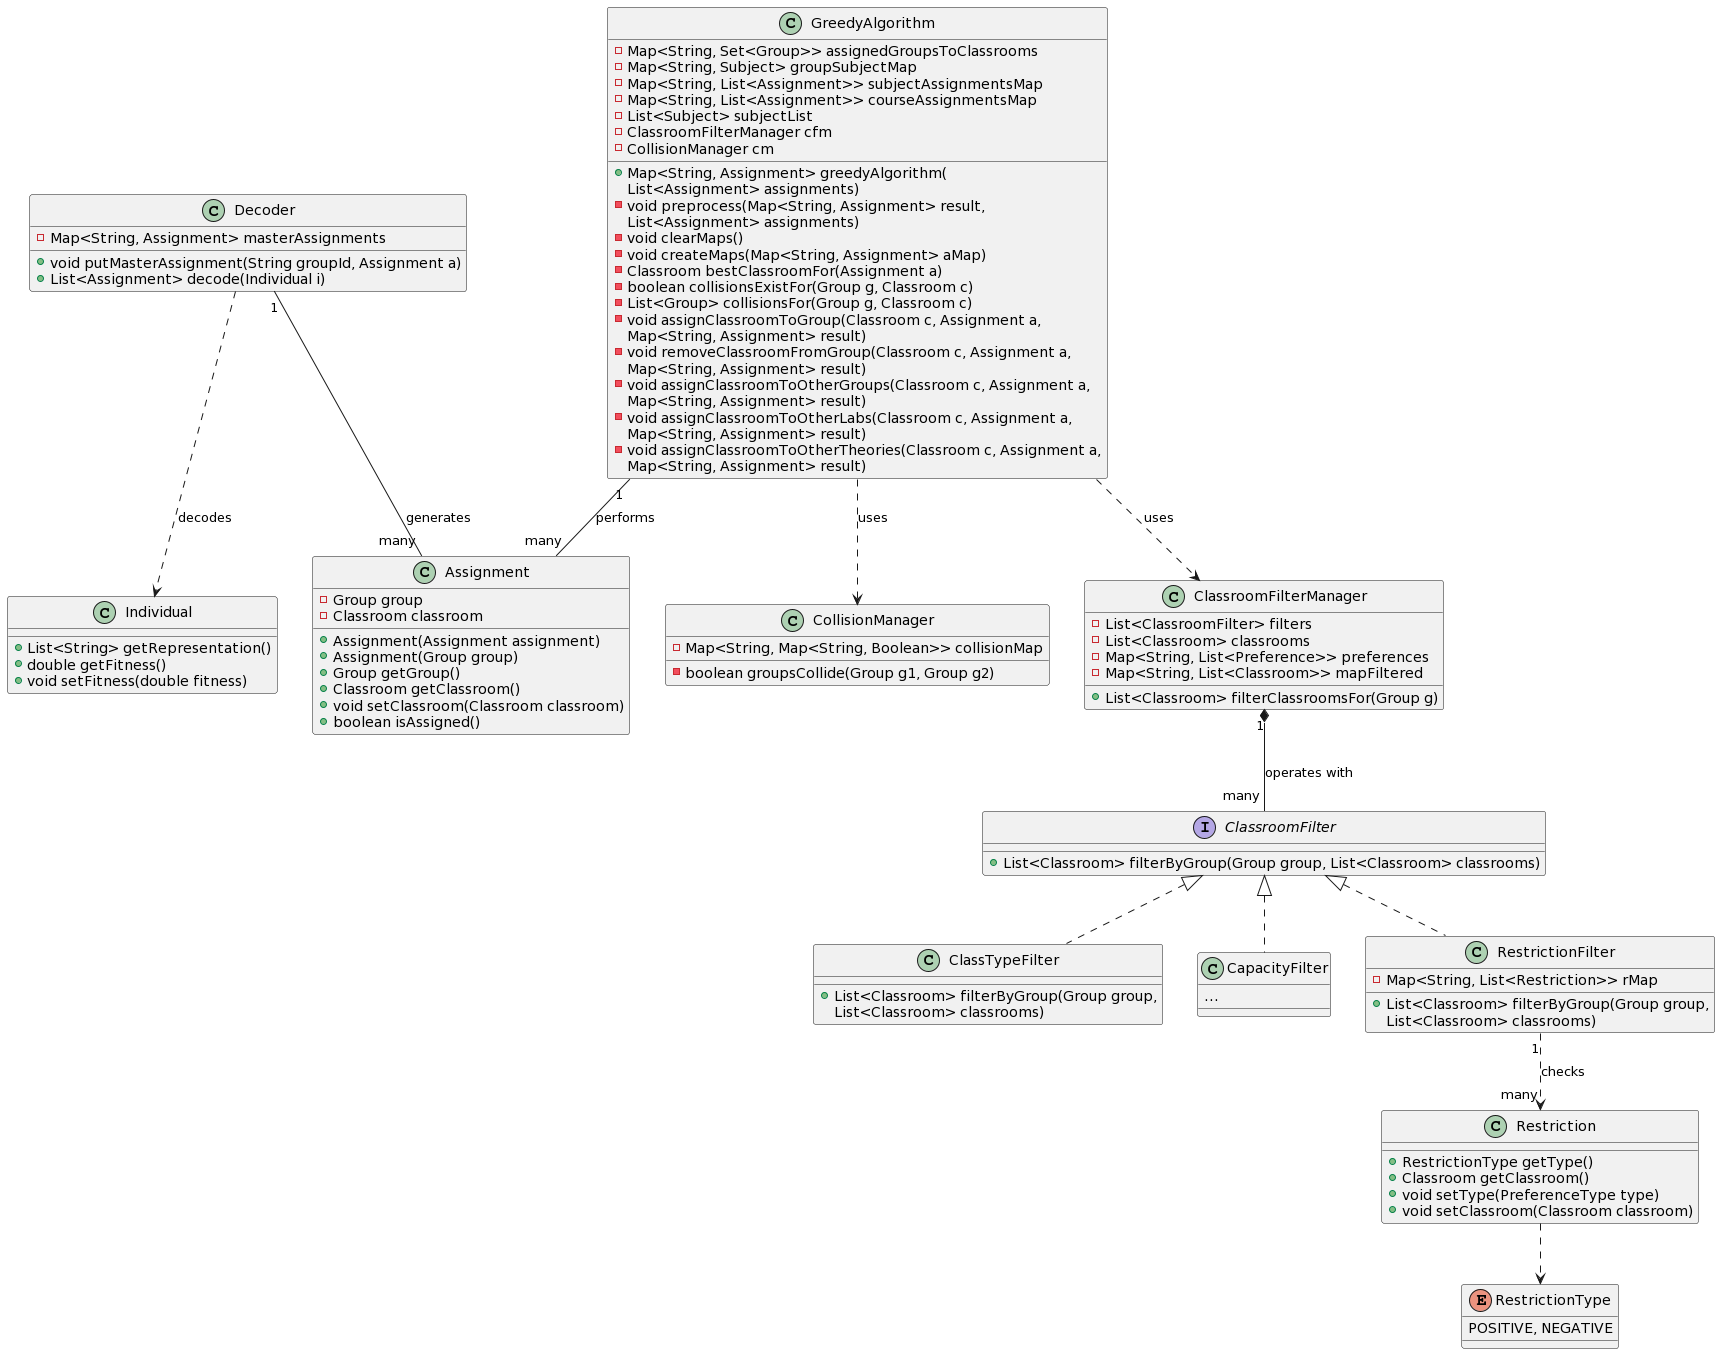
\includegraphics[scale=0.28]{final_alg_greedy_class_diagram_uml.png}
\end{figure}

\begin{figure}[H]
    \caption{Class diagram: Alg package (Genetic algorithm)}
  \centering
  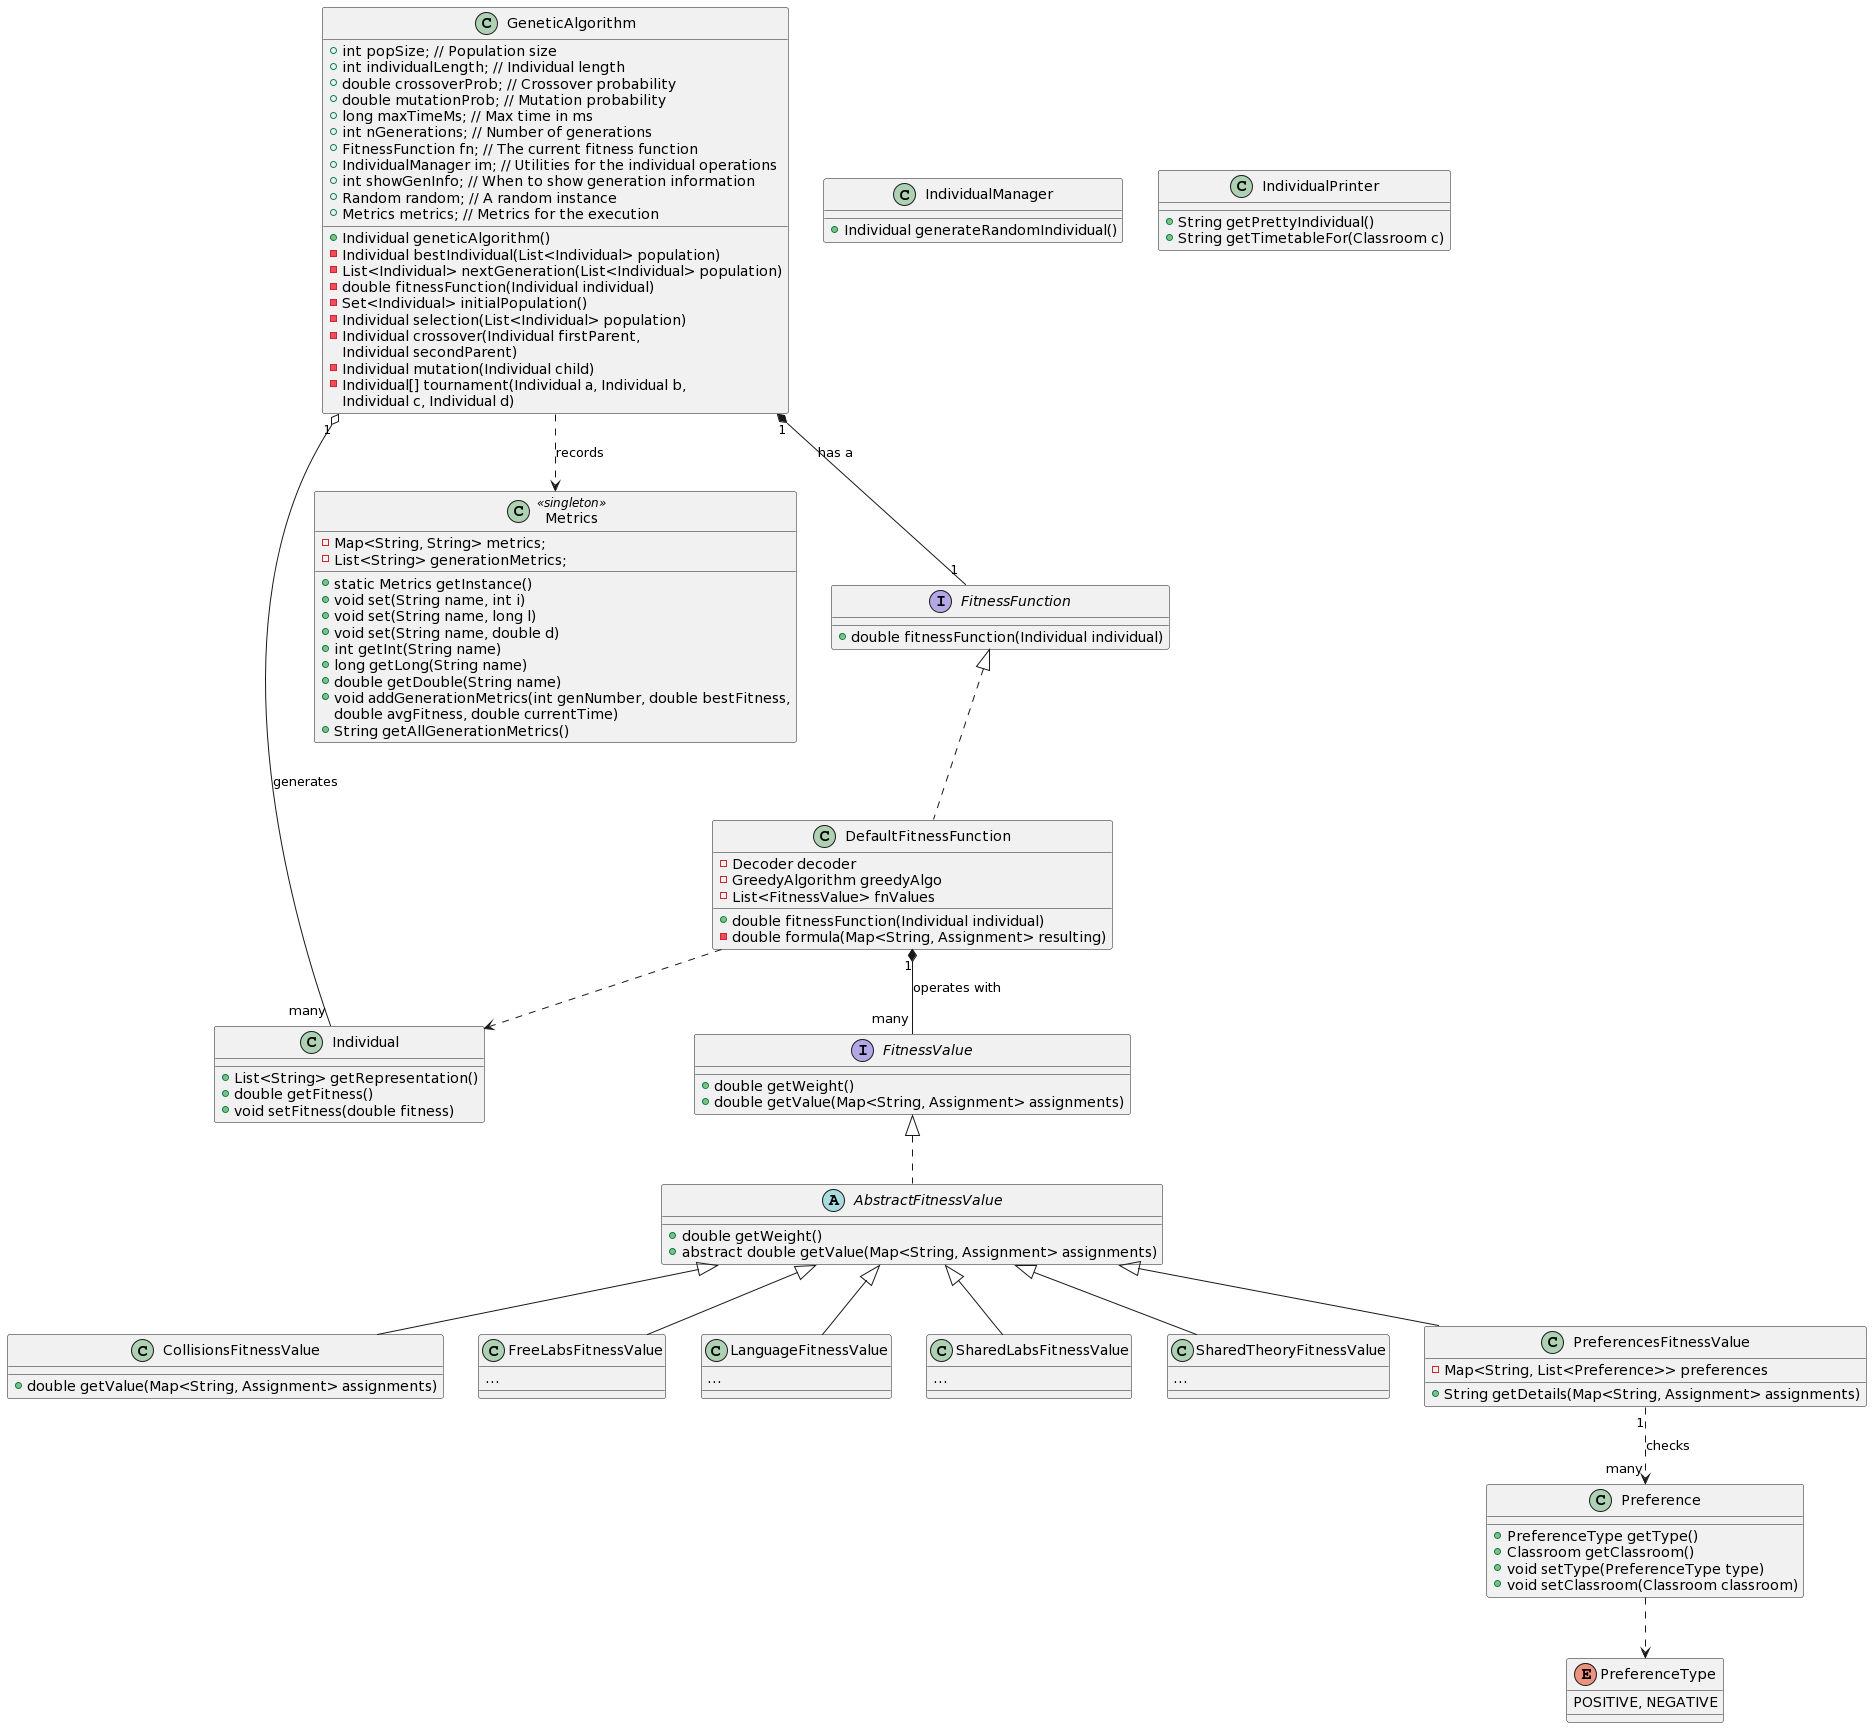
\includegraphics[scale=0.27]{final_alg_genetic_class_diagram_uml.png}
\end{figure}

\begin{figure}[H]
    \caption{Class diagram: Problem domain}
  \centering
  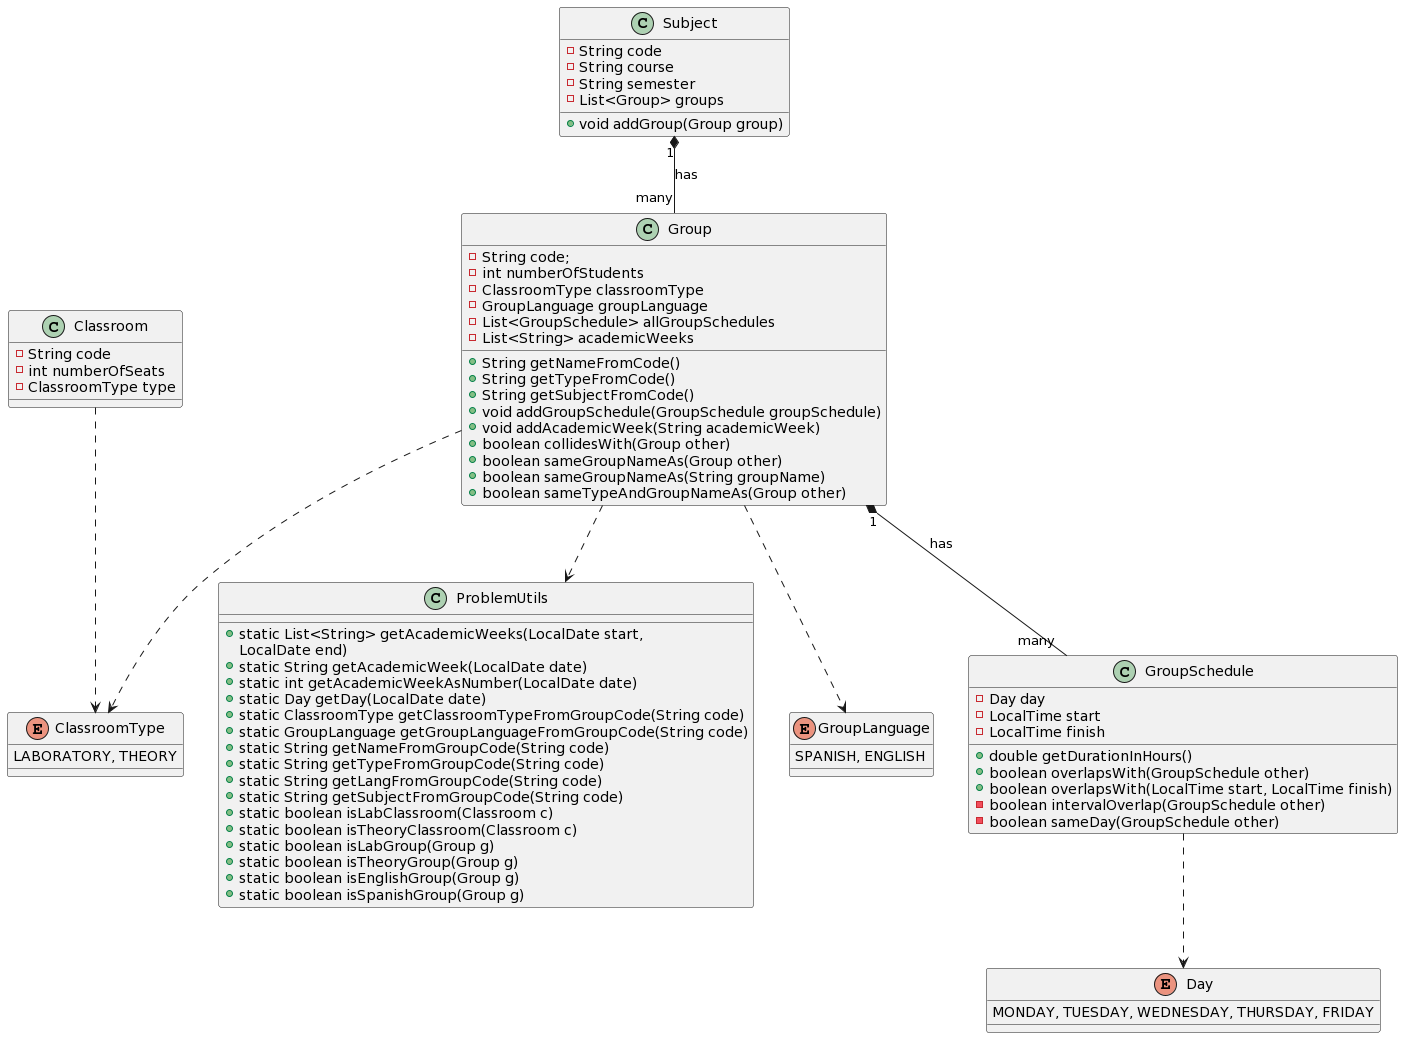
\includegraphics[scale=0.35]{final_problem_class_diagram_uml.png}
\end{figure}

\begin{figure}[H]
    \caption{Class diagram: Other business classes}
  \centering
  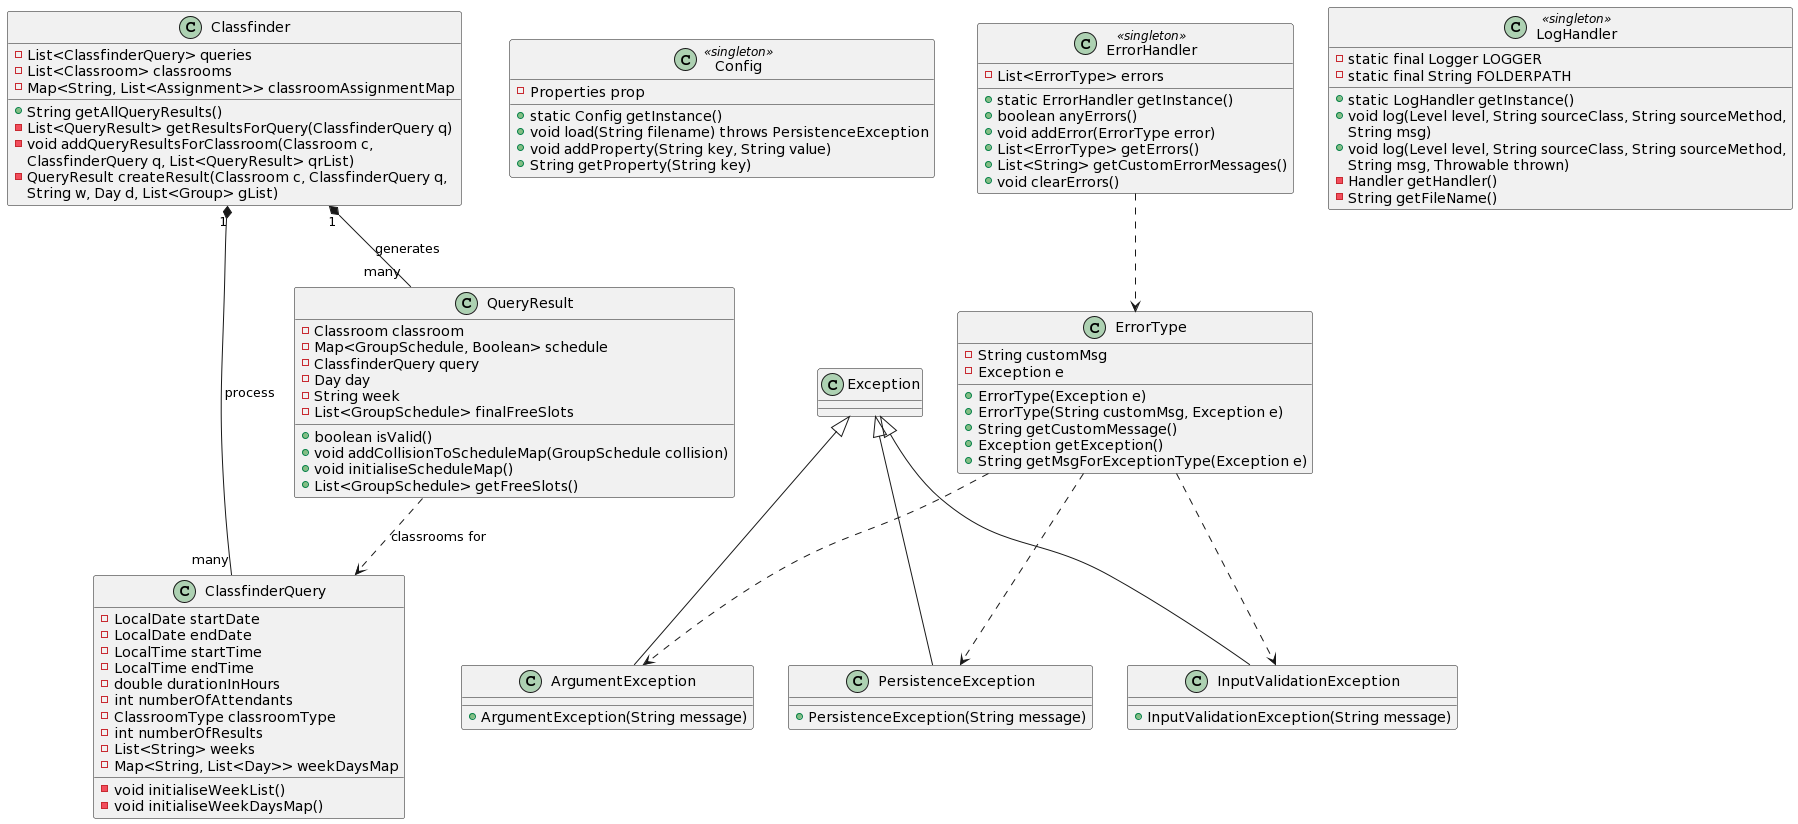
\includegraphics[scale=0.28]{final_business_other_class_diagram_uml.png}
\end{figure}

\begin{figure}[H]
    \caption{Class diagram: Persistence}
  \centering
  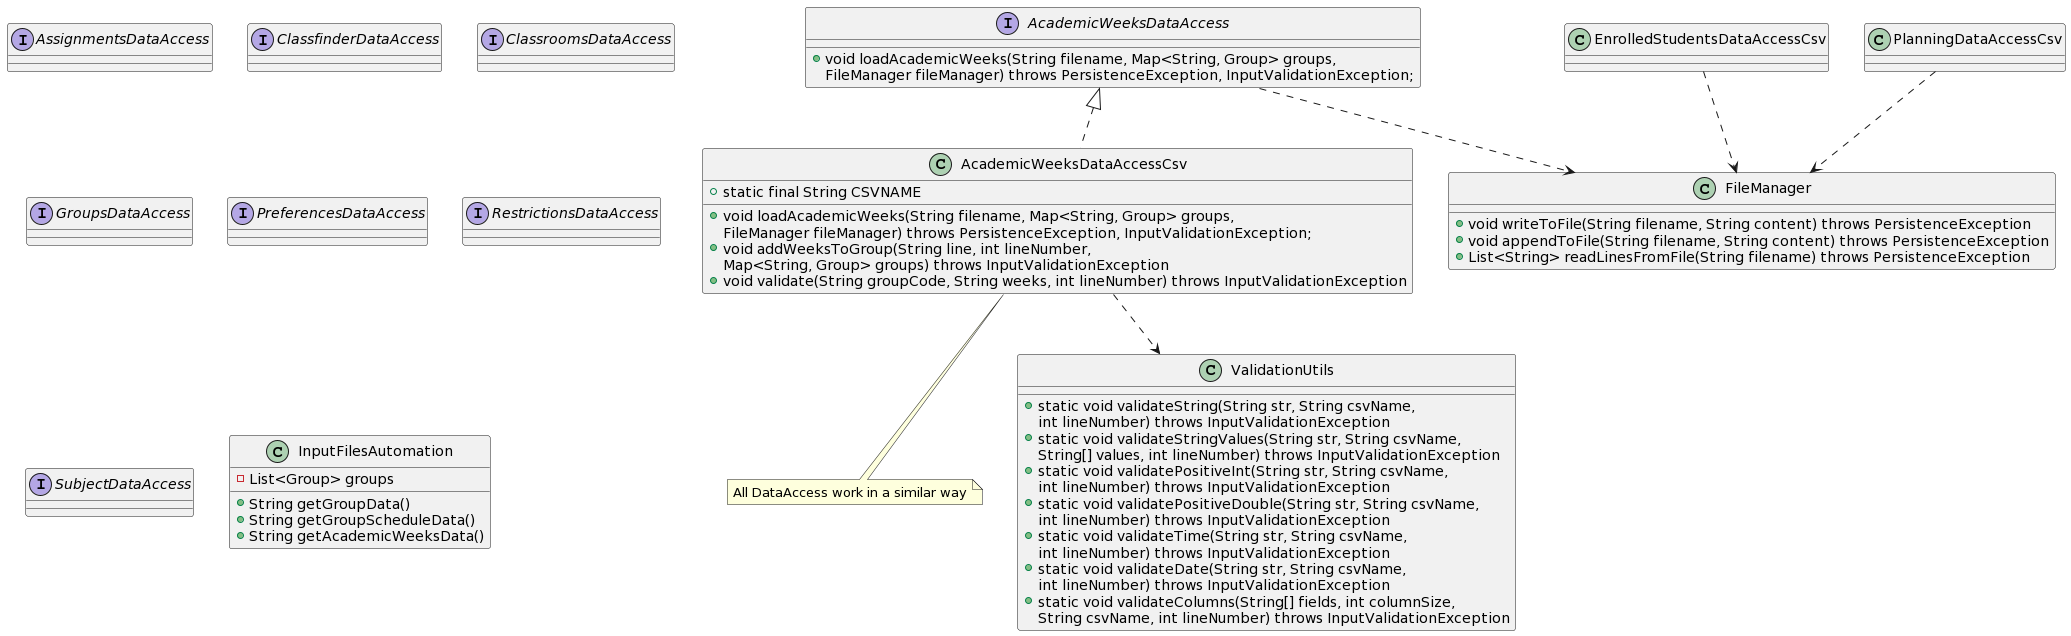
\includegraphics[scale=0.24]{final_persistence_class_diagram_uml.png}
\end{figure}

\begin{figure}[H]
    \caption{Class diagram: Program and CLI}
  \centering
  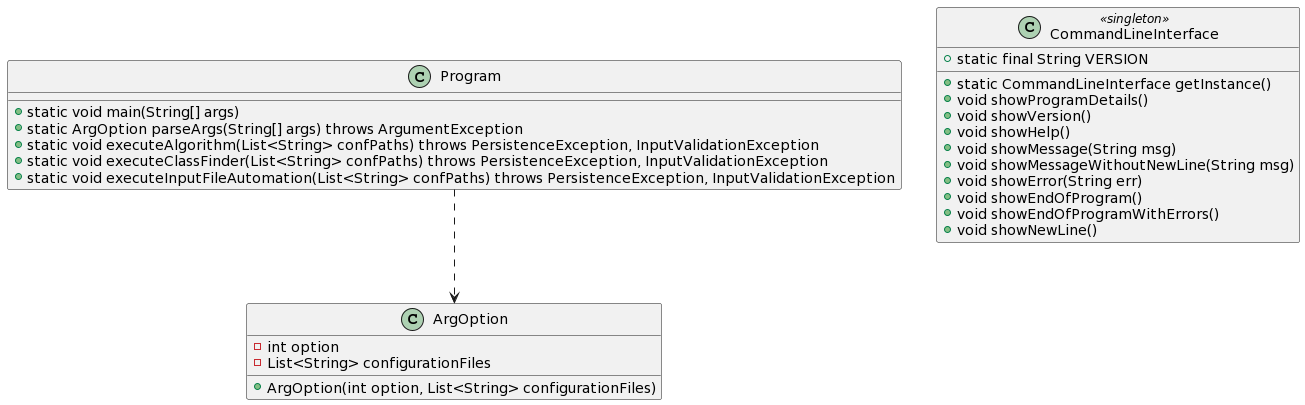
\includegraphics[scale=0.38]{final_main_ui_diagram_uml.png}
\end{figure}


\section{File format design}

We can differentiate files into system files and external files. System files are those that we have originally defined in order for the system to function correctly. External files are those files whose existence precedes this project.

All files are plain text files, and can have the extensions CSV, TXT or PROPERTIES. TXT files contain elements of the solution that are understandable by the user but not processable by the system. CSV and PROPERTIES files are usually input files, in most cases, or output files, in some other cases.

It should be noted that the utility can process as many PROPERTIES files as the user wants. Since these configuration files contain keys and values, the user is free to define them in as many PROPERTIES files as desired, as long as all the required keys are present.

In the case of CSVs, it is expected that these are always separated by semicolons, and that they always include a header with the column names, as the utility always ignores the first line except in special cases. Empty lines will cause errors when parsing, so they must be removed.

All the files involved in the system are now displayed. For real examples, the reader is referred to Annex \ref{annex-file-format}.

Input / Output:

\begin{itemize}
    \item Classrooms (System CSV file)
    \item Subjects (System CSV file)
    \item Groups (System CSV file)
    \item Group schedules (System CSV file)
    \item Group academic weeks (System CSV file)
    \item Preferences (System CSV file)
    \item Restrictions (System CSV file)
    \item Assignments (System CSV file)
    \item Assignments Summary (System TXT file)
    \item Classroom Timetable (System TXT file)
    \item Classfinder queries (System CSV file)
    \item Classfinder query results (System TXT file)
    \item Plan file (External CSV file): It must be manually edited to change the separator to a semicolon and remove its empty lines.
    \item Enrolled students (External CSV file): It must be manually created from the Excel file with the enrolled student tables.
\end{itemize}

Configuration:

\begin{itemize}
    \item Algorithm configuration (System PROPERTIES file): for the \textit{perform the assignments} use case.
    \item Classfinder configuration (System PROPERTIES file): for the \textit{search for free classrooms} use case.
    \item Automation configuration (System PROPERTIES file): for the \textit{automatically create input files} use case.
\end{itemize}

It is again stressed that these configuration files are an agglomeration of all the keys needed for each use case. If the user prefers to split it into other files, as long as they contain all the keys between them, they can do so.

 

    \newpage
    \renewcommand{\documentname}{System implementation}

\chapter{System implementation}


\section{License and references}

\subsection{License}

The software of this project is licensed under the GNU General Public License v2.0.

\subsection{References}

\begin{itemize}
    \item \textit{Java Code Conventions.} Set of guidelines and conventions for programmers to consider when using the Java programming language.

    \item \textit{Linux kernel coding style.} \footnote{Available at \url{https://www.kernel.org/doc/Documentation/process/coding-style.rst}} Set of guidelines and conventions for programmers to consider when programming in the Linux kernel. The stylistic choices in this guide have, for the most part, been the ones adopted for formatting the prototype code, as we believe that the readability of the code is preferable to the Java Code Conventions guidelines.
\end{itemize}



\section{Programming languages}

The use of C or Java for programming the system was discussed. In the end we opted for Java for two reasons. The first is simple, I, the developer, have more experience in Java than in C (although I have used both in this School). Perhaps C would be a suitable language to implement the algorithms described in this document more efficiently, but the extra time I would have to spend learning the language in an advanced way makes it unmanageable for this project. The second reason is also obvious. If this project is to be continued by our colleagues at the School, it would be preferable if it were written in the language that has been learnt throughout the degree courses, i.e, Java.

\section{Tools and programs used in development}

\section{System development}

 

    \newpage
    \renewcommand{\documentname}{Test development}

\chapter{Test development}

As previously stated, the testing phase will focus on checking the correct functioning of the system, especially in the persistence layer. The overall quality of the solutions is assessed in the experimentation stage.

In this chapter, a battery of tests is presented for each use case, each test containing the following information: ID, description, expected outcome, real outcome.



\section{Perform the assignments}

\begin{itemize}
    \item \textbf{ID}: PA-01-NOF
        \begin{itemize}
            \item \textbf{Description}: The utility is executed with a configuration that disables the optional files.
            \item \textbf{Expected outcome}: The assignment process will start from scratch and no restrictions or preferences are to be considered.
            \item \textbf{Real outcome}: OK
        \end{itemize}
    \item \textbf{ID}: PA-02-PREFS
        \begin{itemize}
            \item \textbf{Description}: The utility is executed with a configuration that considers preferences.
            \item \textbf{Expected outcome}: The assignment process will start from scratch and no restrictions are to be considered. Positive and negative preferences will be evaluated as soft constraints.
            \item \textbf{Real outcome}: OK
        \end{itemize}
    \item \textbf{ID}: PA-03-RES
        \begin{itemize}
            \item \textbf{Description}: The utility is executed with a configuration that considers restrictions.
            \item \textbf{Expected outcome}: The assignment process will start from scratch and no preferences are to be considered. Positive and negative restrictions will be evaualted as hard constraints.
            \item \textbf{Real outcome}: OK
        \end{itemize}
    \item \textbf{ID}: PA-04-PAR
        \begin{itemize}
            \item \textbf{Description}: The utility is executed with a configuration that considers a partial list of assignments previously made by the user of the system.
            \item \textbf{Expected outcome}: The assignment process will start from the initial assignments and no preferences or restrictions are to be considered. The initial assignments will remain as they were once the allocation process is completed.
            \item \textbf{Real outcome}: OK
        \end{itemize}
    \item \textbf{ID}: PA-05-CONF
        \begin{itemize}
            \item \textbf{Description}: The utility is executed with a configuration file with missing properties.
            \item \textbf{Expected outcome}: The system will notify the error to the user.
            \item \textbf{Real outcome}: OK
        \end{itemize}
    \item \textbf{ID}: PA-06-INFOR
        \begin{itemize}
            \item \textbf{Description}: The utility is executed with a configuration that points to input files with incorrect format.
            \item \textbf{Expected outcome}: The system will notify the error to the user.
            \item \textbf{Real outcome}: OK
        \end{itemize}
    \item \textbf{ID}: PA-06-INDATA
        \begin{itemize}
            \item \textbf{Description}: The utility is executed with a configuration that points to input files with incorrect information (e.g a group schedule with a reference to a group code that is not present in the system).
            \item \textbf{Expected outcome}: The system will notify the error to the user.
            \item \textbf{Real outcome}: OK
        \end{itemize}
\end{itemize}



\section{Search for free classrooms}

\begin{itemize}
    \item \textbf{ID}: SF-01-THEO
        \begin{itemize}
            \item \textbf{Description}: The utility is executed with a configuration that points to a query file that contains one request for finding a theory classroom.
            \item \textbf{Expected outcome}: The system will look for theory classes that meet the requirements of the query.
            \item \textbf{Real outcome}: OK
        \end{itemize}
    \item \textbf{ID}: SF-02-LAB
        \begin{itemize}
            \item \textbf{Description}: The utility is executed with a configuration that points to a query file that contains one request for finding a laboratory.
            \item \textbf{Expected outcome}: The system will look for laboratories that meet the requirements of the query.
            \item \textbf{Real outcome}: OK
        \end{itemize}
    \item \textbf{ID}: SF-03-ALL
        \begin{itemize}
            \item \textbf{Description}: The utility is executed with a configuration that points to a query file that contains two requests. One to consult free classrooms and another to consult free laboratories. 
            \item \textbf{Expected outcome}: The system will look for theory classrooms for one request and laboratories for the other. Each search must meet the requirements of its associated query.
            \item \textbf{Real outcome}: OK
        \end{itemize}
    \item \textbf{ID}: SF-04-CONF
        \begin{itemize}
            \item \textbf{Description}: The utility is executed with a configuration file with missing properties.
            \item \textbf{Expected outcome}: The system will notify the error to the user.
            \item \textbf{Real outcome}: OK
        \end{itemize}
    \item \textbf{ID}: SF-05-INFOR
        \begin{itemize}
            \item \textbf{Description}: The utility is executed with a configuration that points to input files with incorrect format.
            \item \textbf{Expected outcome}: The system will notify the error to the user.
            \item \textbf{Real outcome}: OK
        \end{itemize}
    \item \textbf{ID}: SF-06-INDATA
        \begin{itemize}
            \item \textbf{Description}: The utility is executed with a configuration that points to input files with incorrect information (e.g a group schedule with a reference to a group code that is not present in the system).
            \item \textbf{Expected outcome}: The system will notify the error to the user.
            \item \textbf{Real outcome}: OK
        \end{itemize}
\end{itemize}



\section{Automatically create input files}

\begin{itemize}
    \item \textbf{ID}: AC-01-AUTO
        \begin{itemize}
            \item \textbf{Description}: The utility is executed with the correct configuration.
            \item \textbf{Expected outcome}: The system will generate the input files necessary for the GA execution.
            \item \textbf{Real outcome}: OK
        \end{itemize}
    \item \textbf{ID}: AC-02-CONF
        \begin{itemize}
            \item \textbf{Description}: The utility is executed with a configuration file with missing properties.
            \item \textbf{Expected outcome}: The system will notify the error to the user.
            \item \textbf{Real outcome}: OK
        \end{itemize}
    \item \textbf{ID}: AC-03-INFOR
        \begin{itemize}
            \item \textbf{Description}: The utility is executed with a configuration that points to input files with incorrect format.
            \item \textbf{Expected outcome}: The system will notify the error to the user.
            \item \textbf{Real outcome}: OK
        \end{itemize}
    \item \textbf{ID}: AC-04-INDATA
        \begin{itemize}
            \item \textbf{Description}: The utility is executed with a configuration that points to input files with incorrect information (e.g a record of enrolled students of a group that does not exist in the planning file).
            \item \textbf{Expected outcome}: The system will notify the error to the user.
            \item \textbf{Real outcome}: OK
        \end{itemize}
\end{itemize}

 

    \newpage
    \renewcommand{\documentname}{Experimental results}

\chapter{Experimental results}\label{experimental-results}

This chapter shows the various experimental studies carried out to evaluate the quality of the prototype and its algorithms. We advance the main thesis we have arrived at after this study: The greedy algorithm is able to solve the problem without the help of the genetic algorithm. However, it is not powerful enough to find the best solutions obtained with other configurations. Only when coupled with the best version of the genetic algorithm does the software perform at its best.


\subsection{Instances}

Four scenarios have been identified for this phase. One scenario is a combination of a group loading level and a constraint loading level. We have groups from the first and second semester of two different academic years, and we have restrictions and preferences obtained from client meetings.

For the charged load level, one group per subject was created for each instance with a 10\% probability, and one restriction or preference with a 20\% probability. Once created, the results were checked for incorrect data or contradictions.

We therefore have the following scenarios:

\begin{itemize}
    \item \textbf{Charged groups - Charged constraints}
    \item \textbf{Charged groups - Regular constraints}
    \item \textbf{Regular groups - Charged constraints}
    \item \textbf{Regular groups - Regular constraints}
\end{itemize}


\subsection{Initial fitness function}

The initial fitness function is created based on the client's expectations of results. The highest weight is given to all assignments being performed, followed by the fulfilment of preferences, then the remaining fitness values.

The values for the initial fitness function follow.

\begin{lstlisting}[basicstyle=\small]
# Fitness weights

# COL_WEIGHT: Weight for the collisions fitness value
COL_WEIGHT = 1.0

# FREE_LABS_WEIGHT: Weight for the free labs fitness value
FREE_LABS_WEIGHT = 0.25

# LANG_WEIGHT: Weight for the group language fitness value
LANG_WEIGHT = 0.25

# SHARED_LABS_WEIGHT: Weight for the shared labs fitness value
SHARED_LABS_WEIGHT = 0.25

# SHARED_THEORY_WEIGHT: Weight for the shared theory classes fitness value
SHARED_THEORY_WEIGHT = 0.25

# PREFS_WEIGHT: Weight for the preferences fitness value
PREFS_WEIGHT = 0.5
\end{lstlisting}



\subsection{Greedy Algorithm reviews}

With this initial fitness function, we proceed to experiment with the following versions of the greedy algorithm:

\begin{itemize}
    \item \textbf{Base greedy}: Algorithm without repairs and biases.
    \item \textbf{Base greedy + Repairs}: Algorithm with repairs but without biases.
    \item \textbf{Base greedy + Repairs + Biases}: Algorithm with repairs and biases towards preferences and shared classrooms.
\end{itemize}


\subsubsection{Fitness reviews}

\subsubsection{Metric reviews}


\subsection{(Genetic + Greedy) parameter reviews}

\subsection{Further fitness functions}

 

    \newpage
    \renewcommand{\documentname}{System manuals}

\chapter{System manuals}


\section{Installation manual}

\subsection*{SETUP}

In order to be able to execute the \textbf{classmanager} utility, two things are required. The first is Java 8 or higher, the second is the creation of the runtime environment. This environment simply consists of having the utility at the same level (in terms of folders) as a folder that the user must create, called \textbf{classmanager\_log}.

\subsection*{FOLDER TREE}

When we run the jar file, we will do it from this folder. If the configuration files have relative paths, they must be relative to the jar file. An example of this is shown below.

\begin{description}
    \item \textbf{Classmanager/} (FOLDER)
        \begin{description}
            \item \textit{classmanager.jar} (Executable JAR)
            \item \textbf{classmanager\_log/} (Required FOLDER)
                \begin{description}
                    \item \textit{Some logs...}
                \end{description}
            \item \textbf{inputfiles/} (User FOLDER)
                \begin{description}
                    \item \textit{classrooms.csv}
                    \item \textit{...}
                \end{description}
            \item \textbf{output/} (User FOLDER)
            \item \textbf{config/} (User FOLDER)
                \begin{description}
                    \item \textit{myConfig.properties}
                \end{description}
        \end{description}
\end{description}

We have the previously described folder in our computer. Let's say we are creating the configuration file \textit{myConfig.properties}, and we want to give a path to the CLASSROOMS\_FILE\_PATH property. Should we specify the relative path from the configuration file or from the jar? As said before, the path is \textbf{relative to the jar file}, so in our case, \verb|CLASSROOMS_FILE_PATH = ./inputfiles/classrooms.csv|.



\section{Execution manual}


\subsection*{NAME}

\begin{description}
    \item classmanager - manages the classrooms and groups of the School of Computing Engineering of Oviedo.
\end{description}


\subsection*{SYNOPSIS}

\begin{description}
    \item \textbf{classmanager} \textit{OPTION} [\textit{FILE...}]
\end{description}


\subsection*{DESCRIPTION}

The \textit{classmanager} utility assigns classes to groups in the School for a given semester. In addition, it allows queries to be made on the classrooms to obtain those available in a range of dates and schedules. Finally, the utility has a built-in tool that allows for automatic conversion of the files currently used by the school into files compatible with the system. 

A \textit{FILE} represents a configuration file. Each option requires a set of properties with values of different types. As long as these properties are given to the utility, the user is free to split them in as many configuration files as they want. If a file is not provided, or if the file cannot be parsed due to lack of permissions, the utility will notify the user of the error. The same goes for the required data not submitted in the configuration files. 


\subsection*{OPTIONS}

\subsubsection*{Generic Program Information}

\begin{description}
    \item \textbf{-h, -{}-help} 
        \begin{description}
            \item Output a usage message and exit.
        \end{description}
    \item \textbf{-v, -{}-version} 
        \begin{description}
            \item Output the version of \textbf{classmanager} and exit.
        \end{description}
\end{description}

\subsubsection*{Functionalities}

\begin{description}
    \item \textbf{-a, -{}-algorithm} 
        \begin{description}
            \item Perform the assignments, output the result into the expected files and exit.
        \end{description}
    \item \textbf{-q, -{}-query} 
        \begin{description}
            \item Search for available classrooms, output the results into the expected files and exit.
        \end{description}
    \item \textbf{-t, -{}-transform} 
        \begin{description}
            \item Transform the School files into compatible files, output the generated files and exit.
        \end{description}
\end{description}


\subsection*{REGULAR EXPRESSIONS}

Three types of regular expressions designed for this project can be used in the \textit{PREFERENCES} and \textit{RESTRICTIONS} files. The three types are taken into account when using them in the name section of a group's code (\textit{subject.type.\textbf{name}}).

The first type involves using the asterisk (*) to indicate that the preference or restriction applies to both English and Spanish groups of a particular type of class (e.g. CVVS.L.*).

The second type uses the addition (+) to indicate that the preference or restriction should apply only to the Spanish groups (e.g. CVVS.L.+).

The last type employs the question mark (?) in the same way as the second type except that the groups concerned are English groups (e.g. CVVS.L.?).


\subsection*{EXIT STATUS}

The program can terminate in two states: \textit{OK} and \textit{ERROR}. The OK status indicates that the execution was completed without problems, while the ERROR status implies that the operation could not be carried out as expected due to an error. The detailed error is recorded in the \textit{LOG} file generated by the utility.


\subsection*{NOTES}

Make sure that all CSV files have a header with the column names, because the program expects such a header to exist. Otherwise it will skip the first row of the CSV. Also, the CSV files cannot have empty rows or the utility will complain. Finally, the utility expects the separator of \textit{all} CSVs to \textit{always} be the semicolon.


\subsection*{COPYRIGHT}

classmanager - manages the classrooms and groups of the School of Computing Engineering of Oviedo.
Copyright (C) 2022  Hugo Fonseca Díaz

This program is free software; you can redistribute it and/or modify
it under the terms of the GNU General Public License as published by
the Free Software Foundation; either version 2 of the License, or
(at your option) any later version.

This program is distributed in the hope that it will be useful,
but WITHOUT ANY WARRANTY; without even the implied warranty of
MERCHANTABILITY or FITNESS FOR A PARTICULAR PURPOSE.  See the
GNU General Public License for more details.

You should have received a copy of the GNU General Public License along with this program; if not, write to the Free Software Foundation, Inc., 51 Franklin Street, Fifth Floor, Boston, MA 02110-1301 USA.


\subsection*{BUGS}


Occasionally an error message will be displayed \textit{after} the message indicating that the program has terminated with error status. It should appear \textit{before} this message. However, repeating the execution may make it appear where expected. 

If you find a bug, you can create an Issue in \href{https://github.com/fonsecadh/classroom-manager-code}{this repository} or send an email to UO258318 AT uniovi DOT es.


\subsection*{EXAMPLES}

Show help:

\verb|java -jar classmanager.jar -h|

\verb|java -jar classmanager.jar --help|

Show version:

\verb|java -jar classmanager.jar -v|

\verb|java -jar classmanager.jar --version|

Performing the assignments:

\verb|java -jar classmanager.jar -a algFolder/algorithm.properties|

\verb|              ioFolder/io.properties|

Note that the user has decided to split the properties in two files, but they could have used only one if they wanted.

Another way of performing the assignments:

\verb|java -jar classmanager.jar --algorithm all.properties|

Searching for classrooms:

\verb|java -jar classmanager.jar -q classfinder.properties|

\verb|java -jar classmanager.jar --query one.properties|

\verb|              two.properties three.properties|

Transforming the files of the School into the files used by the utility:

\verb|java -jar classmanager.jar -t automation.properties|

\verb|java -jar classmanager.jar --transform automation.properties|



\subsection*{SEE ALSO}

You can view the updated documentation at \href{https://github.com/fonsecadh/classroom-manager-doc}{this repository}. If you wish to view the code, you can do so by visiting \href{https://github.com/fonsecadh/classroom-manager-code}{this other repository}.



\section{User manual}

This manual explains the different files involved in the three possible use cases. See Annex \ref{annex-file-format} for examples of each use case.


\subsection*{PERFORM THE ASSIGNMENTS}


\subsubsection*{CONFIG}

A default configuration is provided for the greedy algorithm and for the genetic algorithm. The only notable thing about this property file is that you can specify the path to the optional files but disable their use with boolean keys.

\subsubsection*{INPUT}

Files submitted for classes and subjects can be reused. It is important to keep the headers of each CSV file and not to have empty rows, as discussed in the execution manual. 

If a group or subject code is referenced in another csv file, a check will be made to see if that code exists. However, the codes will not be checked to see if they are well-formed in the original files, so special care must be taken.

The format of dates and times should also be taken into account, so it is recommended to study the files already submitted for reference. The utility will check if they are incorrectly formatted and will warn the user of any problems.

If you start from an existing mapping file, note that there can be no classless mappings or the utility will interpret this as an error when parsing the file.


\subsubsection*{OUTPUT}

Several types of files are generated. It can be categorised into three types, the csv file of assignments, the txt file with the summary of assignments and the files with the timetable in tabular form.

The summary file indicates first the assignments without a class, then the groups whose assignments do not meet the preferences, and finally the assignments sorted by course and subject.

The timetables show in table format the timetable of each class. If there is more than one group in a cell, it means that both groups have the same time, but it is understood that they never overlap in their academic weeks.


\subsection*{SEARCH FOR FREE CLASSROOMS}


\subsubsection*{INPUT}

As the queries are entered via CSV, as many queries as the user wants can be introduced. Care should be taken not to enter a start date that is later than the end date.

\subsubsection*{OUTPUT}

A txt file is generated. This file contains, for each query, its parameters and results. The results include a class, a week, a day and a series of ranges of free slots for that classroom.



\subsection*{AUTOMATICALLY CREATE INPUT FILES}


\subsubsection*{INPUT}

Input files must be correctly adapted to the system. This involves using the semicolon separator and deleting all empty lines. A header must also be created for both files (see example files provided in the Annex).

\subsubsection*{OUTPUT}

The group, group schedules and group academic weeks are generated. Since the system does not contain the subjects in memory for this use case, the entries are sorted by the code of the groups.




\section{Programmer manual}


\subsection*{LOG}

\begin{lstlisting}[basicstyle=\tiny]
DETALLADO: START Persistence logic
jul 05, 2022 12:23:15 AM main.Program main
GRAVE: Wrong integer in GROUPS csv file (cero or negative: 0), line 42
business.errorhandler.exceptions.InputValidationException: Wrong integer in GROUPS csv file (cero or negative: 0), line 42
	at persistence.problem.csv.utils.ValidationUtils.validatePositiveInt(ValidationUtils.java:56)
	at persistence.problem.csv.GroupsDataAccessCsv.validate(GroupsDataAccessCsv.java:106)
	at persistence.problem.csv.GroupsDataAccessCsv.lineToGroup(GroupsDataAccessCsv.java:51)
	at persistence.problem.csv.GroupsDataAccessCsv.loadGroups(GroupsDataAccessCsv.java:29)
	at main.Program.executeExperiments(Program.java:855)
	at main.Program.main(Program.java:94)

jul 05, 2022 12:24:50 AM main.Program main
DETALLADO: START Persistence logic
jul 05, 2022 12:24:50 AM main.Program main
GRAVE: Non existing code for group in PREFERENCES csv file (CPM.L.+), line 6
business.errorhandler.exceptions.InputValidationException: Non existing code for group in PREFERENCES csv file (CPM.L.+), line 6
	at persistence.problem.csv.PreferencesDataAccessCsv.lineToPreferences(PreferencesDataAccessCsv.java:97)
	at persistence.problem.csv.PreferencesDataAccessCsv.loadPreferences(PreferencesDataAccessCsv.java:34)
	at main.Program.executeExperiments(Program.java:883)
	at main.Program.main(Program.java:94)

jul 05, 2022 12:25:21 AM main.Program main
DETALLADO: START Persistence logic
jul 05, 2022 12:25:21 AM main.Program main
DETALLADO: END Persistence logic
jul 05, 2022 12:25:21 AM main.Program main
DETALLADO: START Business logic
jul 05, 2022 12:25:21 AM business.alg.gen.logic.GeneticAlgorithm geneticAlgorithm
DETALLADO: START Genetic Algorithm
jul 05, 2022 12:25:21 AM business.alg.gen.logic.GeneticAlgorithm geneticAlgorithm
MUY DETALLADO: Parameters:

	-> Max number of generations: 10
	-> Max time (ms): 360000
	-> Mutation probability: 0.5
	-> Crossover probability: 0.9
	-> Population size: 200
	-> Fitness function: business.alg.gen.logic.fitness.DefaultFitnessFunction
	-> Individual length: 311
jul 05, 2022 12:25:29 AM business.alg.gen.logic.GeneticAlgorithm geneticAlgorithm
DETALLADO: END Genetic Algorithm
jul 05, 2022 12:25:29 AM main.Program main
DETALLADO: END Business logic
\end{lstlisting}

The above is an extract from the log file. We can see a trace of the flow of the application in three different executions. The first two fail, each with a different error, in the groups and preferences files. The last one occurs after the errors have been fixed and the parameters of the genetic algorithm used for the execution can be observed. Once the execution of the genetic is finished, an entry indicating this fact and another one reporting the completion of the business logic are created.



\subsection*{UTILITIES}

CSV and problem domain validation utilities can be used to lighten and de-code new implementations.

If a new exception type is to be introduced, it must be defined in the business layer error handler package and specified as an expected exception by instructing the ErrorType.



\subsection*{NOTES}

Some notes follow.

\begin{itemize}
    \item New use cases should be executed in the Program class as a unique function with a series of steps (see the other use cases).
    \item All printing to the terminal must be via the CommandLineInterface class.
    \item Changes to the problem domain classes and to the utility classes should be reviewed carefully, as much of the system depends on such classes. 
    \item If more GA operators are to be developed, a Strategy Design Pattern approach, similar to the FitnessFunction, is recommended.
    \item New fitness values for the GA should follow the current procedure of returning a value between 0 and 100.
    \item If data collections are shared between objects, copies of the collections must be shared. If the objects in these collections are to be modified, the shared collection must contain cloned objects (this can be seen in the Decoder class).
\end{itemize}


 

    \newpage
    \renewcommand{\documentname}{Conclusions}

\chapter{Conclusions}

\section{Future work}
\section{Final conclusions}

 

    \newpage
    \renewcommand{\documentname}{Budget}

\chapter{Budget} \label{section-budget}

This chapter presents the budget for the work. First the internal budget will be calculated taking into account the environment in which we work, and then the budget of the client will be prepared with the necessary items and the benefits applied.

The working time concept is reiterated. Each week has seven working days of three hours each. It is important to bear in mind this concept of working day in order to understand some sections of the budget.

\section{Internal budget}

To calculate the internal budget we must first define our situation. We are two freelancers, a junior and a senior software engineer (see Figure \ref{fig-budget-workers}).


\begin{figure}[H]
    \caption{Freelancers description}
    \label{fig-budget-workers}
  \centering
  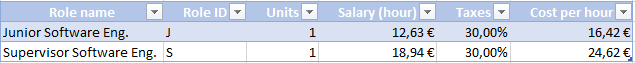
\includegraphics[scale=1]{budget_workers.PNG}
\end{figure}

We have the following rental and amortisation expenses related to the project (see Figure \ref{fig-budget-amortisations}).


\begin{figure}[H]
    \caption{Amortisation costs}
    \label{fig-budget-amortisations}
  \centering
  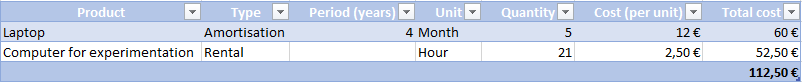
\includegraphics[scale=0.8]{budget_amortisations.PNG}
\end{figure}

Indirect costs are shown below (see Figure \ref{fig-budget-ic}).


\begin{figure}[H]
    \caption{Indirect costs}
    \label{fig-budget-ic}
  \centering
  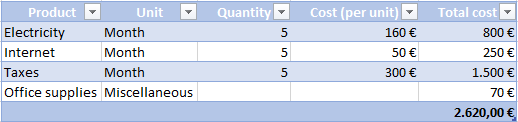
\includegraphics[scale=1]{budget_indirect_costs.PNG}
\end{figure}

Finally, we calculate the costs of carrying out the tasks defined in the WBS.


\begin{figure}[H]
    \caption{WBS Budget costs: Project Management and Analysis}
    \label{fig-budget-wbs-01}
  \centering
  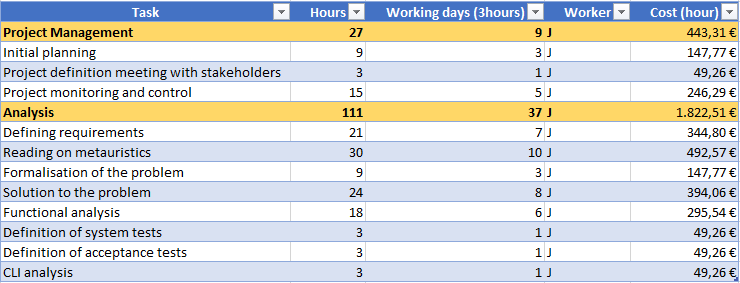
\includegraphics[scale=0.7]{budget_wbs_01.PNG}
\end{figure}


\begin{figure}[H]
    \caption{WBS Budget costs: Design and Development}
    \label{fig-budget-wbs-02}
  \centering
  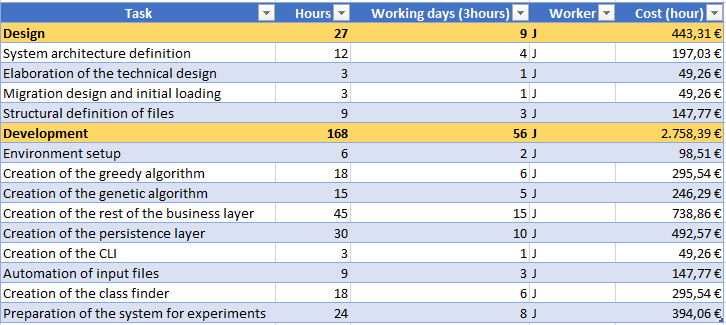
\includegraphics[scale=0.7]{budget_wbs_02.PNG}
\end{figure}


\begin{figure}[H]
    \caption{WBS Budget costs: Documentation, Experiments and Closure}
    \label{fig-budget-wbs-03}
  \centering
  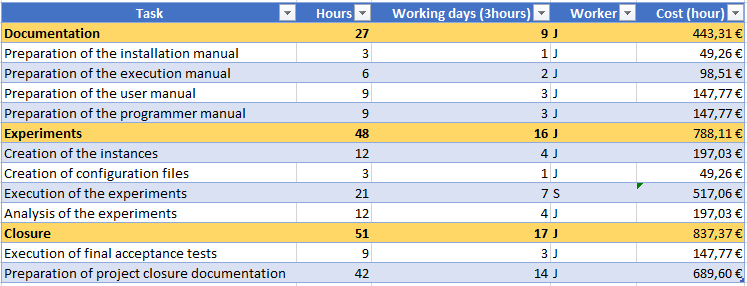
\includegraphics[scale=0.7]{budget_wbs_03.PNG}
\end{figure}

So we are left with the following cost of the WBS phases (see Figure \ref{fig-budget-wbs-sum}).


\begin{figure}[H]
    \caption{WBS Budget costs: Summary}
    \label{fig-budget-wbs-sum}
  \centering
  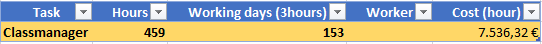
\includegraphics[scale=0.7]{budget_wbs_04.PNG}
\end{figure}

With the addition of all the costs calculated so far, we obtain the internal budget for the project.


\begin{figure}[H]
    \caption{Internal budget}
    \label{fig-budget-internal}
  \centering
  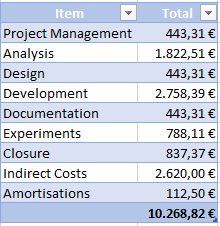
\includegraphics[scale=1]{budget_internal.PNG}
\end{figure}



\section{Client budget}


This project is expected to yield a profit of 25\%. With this information we will proceed to calculate the client's budget. It is important to note that the client will not be shown a budget with all the items, only the generic ones that describe the work to be done. Therefore, we must calculate the amount of the items not shown added to the benefits, and thus obtain a weighting value with which to calculate the client's final budget.

Figure \ref{fig-budget-weight} demonstrates the calculation of this weighting value.


\begin{figure}[H]
    \caption{Weighting value calculation}
    \label{fig-budget-weight}
  \centering
  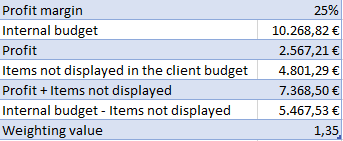
\includegraphics[scale=1]{budget_weighting.PNG}
\end{figure}

Each item is added to its own value multiplied by the weighting value and entered into the client's final budget (See Figure \ref{fig-budget-client}). This means that a cost $c_{i}$ shown in the internal budget will be transformed into a new cost if the item appears in the client budget. This transformation is given by $x_{i} = c_{i} + c_{i} w$, where $w$ is the weighting value. 


\begin{figure}[H]
    \caption{Client budget}
    \label{fig-budget-client}
  \centering
  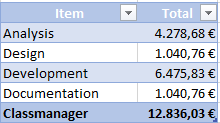
\includegraphics[scale=1]{budget_client.PNG}
\end{figure}




 

    \newpage
    \renewcommand{\documentname}{Annexes}

\chapter{Annexes}


\section{Definitions and abbreviations}

\section{Submission contents}

 

    \newpage
    \renewcommand{\documentname}{Bibliography}

\chapter{Bibliography}

\section{TODO}

TODO



    \newpage
    
% Back cover
\includepdf[pages=2]{other/covers.pdf}



}

\renewcommand{\documentname}{Bibliography}

\end{document}

